\documentclass[12pt,a4paper]{ctexrep}

% --- 宏包 ---
\usepackage{geometry,setspace,titlesec,fancyhdr}
\usepackage{amsmath,amssymb,booktabs,tabularx,graphicx}
\usepackage{enumitem}
\usepackage[hidelinks]{hyperref}
\usepackage{tikz,float}
\numberwithin{equation}{section}
\usetikzlibrary{shapes.geometric, arrows, positioning, calc}

% --- 页面边距与布局 ---
\geometry{top=2.5cm,bottom=2.54cm,left=2.5cm,right=2.5cm}

% --- 字体设置 ---
\setCJKmainfont{SimSun}
\setCJKsansfont{SimHei}
\setmainfont{Times New Roman}
\newcommand{\song}{\songti}
\newcommand{\hei}{\heiti}

% --- 段落与页眉页脚 ---
\setlength{\parskip}{0pt}
% --- 页眉页脚设置 ---
\pagestyle{fancy}
\fancyhf{}
\cfoot{\song\footnotesize\thepage}
\renewcommand{\headrulewidth}{0pt}


% --- 重新定制标题格式 ---
\titleformat{\section}[block]{\hei\zihao{-3}}{\thesection}{1em}{}
\titlespacing{\section}{0pt}{8pt}{8pt}

\titleformat{\subsection}[block]{\hei\zihao{4}}{\thesubsection}{1em}{}
\titlespacing{\subsection}{0pt}{5pt}{5pt}

\titleformat{\subsubsection}[block]{\hei\zihao{4}}{\thesubsubsection}{1em}{}
\titlespacing{\subsubsection}{0pt}{5pt}{5pt}

\renewcommand{\thesection}{\arabic{section}}
\renewcommand{\thesubsection}{\thesection.\arabic{subsection}}
\renewcommand{\thesubsubsection}{\thesubsection.\arabic{subsubsection}}
\setcounter{secnumdepth}{3}

% --- 引用符号定制（上标、带中括号） ---
\newcommand{\citeup}[1]{\textsuperscript{[#1]}}


\begin{document}
	% 前置部分：中文摘要 
	\newpage
	\pagenumbering{arabic} % 设置阿拉伯数字页码
	
	% --- 1. 中文摘要 ---
	\begin{center}
		{\hei\zihao{2}基于孕妇级验证的NIPT检测时点优化与女胎异常判定}
	\end{center}
	\noindent{\hei\zihao{-3}摘要}\par
	\vspace{11pt}
	
	\begin{spacing}{1.0}
		{\song\zihao{4} \setlength{\parindent}{2em}
			NIPT检测是当下检验胎儿是否健康的有效手段，但其面临如下问题：过早可能因胎儿游离DNA不足而失败，过晚又会压缩后续诊疗窗口，因此检测时点直接关系筛查的可靠性与处置风险。本文以孕妇为独立单位，系统解决Y染色体浓度关系辨识、男胎首检--重检时点优化与女胎异常判定问题，并明确各结论的适用边界。

			数据预处理采用“原值保留、确定性补缺、争议样本标记、技术复测成组”的统一口径，并以复测组中位数及左删失、区间删失、右删失重构稳健观测与首次达标信息。进一步设计{\hei\bfseries 以孕妇为单位的嵌套验证}：男胎{\hei\bfseries 267名孕妇、1082条记录}与女胎{\hei\bfseries 147名孕妇、605条记录}分别划分开发集和锁定测试集；同一孕妇及复测组不跨集合，插补、筛选、调参、时点与阈值均仅在内层训练折确定，下游只接收折外结果，从源头阻断同人跨折和测试集回流。

			问题一采用{\hei\bfseries Mundlak组内--组间分解}及孕妇聚类稳健推断。同一孕妇内孕周每增加1周，Y染色体浓度平均增加{\hei\bfseries 0.003203}（Holm校正$p<0.001$）；孕妇间平均BMI每增加$1\,\mathrm{kg/m^2}$，Y浓度平均降低{\hei\bfseries 0.001819}（校正$p=0.049$）。锁定测试中三个核心效应方向保持一致，但记录级$R^2$仅为{\hei\bfseries 0.253}，故该模型用于关系解释而非个体浓度预测。

			问题二、三经{\hei\bfseries 孕妇级五折增量验证、one-SE规则与预设升级门槛}，确认第三问与问题二采用同一冻结基线；随后以{\hei\bfseries 有序收缩Logistic达标概率模型}估计$Y\geq4\%$的概率，并接入{\hei\bfseries 检测--重检风险函数与有限网格优化}。BMI划为$<30$、$[30,35)$和$\geq35$三个风险沟通层，数据不支持三组使用不同概率曲线；加入年龄、身高、体重、受孕方式和孕产史后，最佳候选Brier分数仅改善{\hei\bfseries 2.06\%}，未达到升级线，故两问采用同一策略。基准情景下三组均于{\hei\bfseries 10.5周首检、11.0周重检}，累计可靠概率为{\hei\bfseries 0.9009}；{\hei\bfseries 192个预设情景}中136个可行，最优首检周覆盖{\hei\bfseries 10--22.5周}，经1000次联合bootstrap仅{\hei\bfseries 56个情景}稳定，故单点时点仅是给定误差、重检成功率与风险权重下的条件解。

			问题四以AB列为标签，建立含13、18、21和X染色体Z值、X染色体浓度及GC含量的{\hei\bfseries $L_2$加权Logistic模型（M2）}。计算异常分数$p$后，$p<\mathbf{0.471680}$判为正常倾向，$p>\mathbf{0.747108}$判为异常倾向，中间区间转入复核；二分类评价阈值为{\hei\bfseries 0.635314}。锁定测试{\hei\bfseries PR-AUC为0.175606、召回率为0.384615}，表明该规则只能复现当前附件平台的AB标签，不能替代临床诊断。

			本文以{\hei\bfseries 孕妇级防泄漏划分}$\rightarrow${\hei\bfseries 预设升级裁决}$\rightarrow${\hei\bfseries 折外冻结模型}$\rightarrow${\hei\bfseries 情景枚举与bootstrap}$\rightarrow${\hei\bfseries 锁定测试及灰区/不可行输出}构成闭环证据链。该“关系辨识--概率估计--条件决策--边界审计”流程，可复用于具有重复测量、阈值达标、重检路径和少数类判定的生物标志物研究。
		}
	\end{spacing}
	
	\vspace{1em}
	\noindent{\hei\zihao{4}关键词：无创产前检测；重复测量；达标概率；风险优化；异常判定}
	
	\newpage
	
	% 正文部分
	\begin{spacing}{1.10}
		{\song\zihao{-4}
		%引言部分
			\section{问题背景}
			%简要概括这个研究目标的重要性
			NIPT通过分析孕妇外周血中的胎儿游离DNA，对13、18和21号染色体非整倍体风险进行筛查。检测过早时，胎儿来源DNA比例可能不足；检测过晚又会压缩后续复核和干预时间。母体BMI、孕周及测序质量均可能改变可获得可靠结果的概率，且这种影响依赖具体人群和检测平台\citeup{1,7,13}。因此，检测时点的选择本质上是可靠性、等待风险与重检成本之间的条件决策，而非寻找一个适用于所有孕妇的固定孕周。

			附件数据还包含同一孕妇的多次采血和同次采血复测。若把每条记录视为独立样本，个体差异会被重复计数，模型选择和测试性能也会因信息泄露而偏高。女胎异常记录较少，AB标签在部分复测组内不一致，进一步限制了复杂分类器的可用性。本文据此把孕妇作为数据划分和不确定性评估的基本单位，并在所有问题中保留技术复测、删失信息和质量标记。
			
			%简要概括问题的具体是什么，转化数学建模目标
			围绕题目给出的四项任务，本文将研究目标转化如下：
			\begin{enumerate}[label=\arabic*),itemsep=2pt,topsep=2pt]
			\item 分离同一孕妇随孕周变化的组内效应与不同孕妇之间的组间差异，建立Y染色体浓度关于孕周、BMI及其交互的关系模型，并给出聚类稳健显著性检验；
			\item 以$Y\geq4\%$定义男胎检测达标，估计各孕周的达标概率；在BMI分层下联合考虑首次检测、至多一次重检、检测误差和延迟损失，求解条件最优NIPT时点；
			\item 在问题二的概率--风险框架中加入年龄、身高、体重、受孕方式和孕产史等因素，检验这些信息能否稳定改变BMI分组或检测时点，并分析误差参数对策略的影响；
			\item 以女胎AB列是否非空构造异常标签，综合染色体Z值、X染色体浓度和测序质量特征，输出可复算的异常分数、判定阈值及不确定灰区。
			\end{enumerate}
			
			\section{问题分析}
			首先，附件中的“一行检测记录”不能被视为一个独立样本：同一孕妇可能在不同孕周多次采血，同次采血又可能产生技术复测，各记录共享未观测的个体基础状态。若忽略这种层级结构，检测次数较多的孕妇会被重复赋权，标准误和验证成绩也会被人为放大。与此同时，Y染色体浓度在个体内并非严格单调，横截面上孕周、BMI与个体差异又相互混杂，故必须区分“同一孕妇随时间的变化”与“不同孕妇之间的差异”，不能把二者压缩成一条总体相关线。

			数据质量和任务标签还带来第二层限制。缺失值中既有可由身高、体重确定性补算的BMI，也有因胎儿性别而产生的结构性空白；极端BMI、GC离群和读段冲突可能是真实风险或质量信号，不能统一删除。男胎的首次达标时间只被有限次检测夹在左删失、区间删失或右删失范围内，首条阳性记录并不等于真实达标时点。女胎AB标签类别不平衡，且部分技术复测的标签不一致；题目也未提供独立确诊标签、完整重抽结局和临床误判代价。

			据此，一些直观方法并不适用。逐行建立多元线性回归会违反观测独立性，并混淆组内与组间效应；直接对BMI做K-means或层次聚类，只能按样本分布形成几何分组，在两端样本稀少时切点容易漂移，也不能保证分组真正对应检测风险差异。把首条阳性当作精确事件再拟合普通生存模型，或对非单调Y浓度作线性插值，都会制造数据中不存在的达标时点。按记录随机划分训练集和测试集会使同一孕妇的信息跨集合泄漏；在异常样本有限时直接堆叠高维非线性分类器，或以准确率选模型，则容易得到偏向多数类的表面高分。类似地，用一组未经题目给定的损失权重直接求唯一最优孕周，会把主观假设包装成精确结论。

			因此，后续建模采用如下统一的框架：先按孕妇组织数据，保留技术复测、删失区间和质量标记，再通过孕妇级开发集、内层验证与锁定测试隔离模型选择和最终评价。问题一以关系解释为目标，优先处理重复测量相关性并分离个体内外效应；问题二将“达标规律的估计”与“检测--重检决策”分层，只有分组带来稳定增益时才采用差异化时点；问题三在同一基线上检验新增因素，证据不足时不增加模型复杂度；问题四围绕少数类、共线性和阈值不确定性控制模型容量，并允许输出灰区。题目无法识别的误差、重检成功率和损失权重进入预设情景与bootstrap，最终只报告经锁定测试支持的结论及其适用边界。总体思路见图\ref{fig:overall_flow}。

			\begin{figure}[H]
			\centering
			\begin{tikzpicture}[
				box/.style={draw,rounded corners,align=center,minimum height=1.05cm,text width=2.75cm,font=\small},
				wide/.style={draw,rounded corners,align=center,minimum height=1.0cm,text width=4.1cm,font=\small},
				arr/.style={->,>=stealth,thick}
			]
			\node[wide] (raw) at (-2.7,2.0) {识别数据风险\\重复、删失、缺失与不平衡};
			\node[wide] (prep) at (2.7,2.0) {统一分析单位与验证边界\\复测成组、孕妇级防泄漏};
			\node[box] (q1) at (-5.25,-0.1) {问题一\\纵向关系与相关性};
			\node[box] (q2) at (-1.75,-0.1) {问题二\\概率估计与条件决策};
			\node[box] (q3) at (1.75,-0.1) {问题三\\新增因素的增量证据};
			\node[box] (q4) at (5.25,-0.1) {问题四\\少数类判定与灰区};
			\node[wide] (out) at (0,-2.25) {锁定测试与稳健性分析\\输出结论及适用边界};
			\draw[arr] (raw) -- (prep);
			\draw[arr] (prep.south) |- (q1.north);
			\draw[arr] (prep.south) |- (q2.north);
			\draw[arr] (prep.south) |- (q3.north);
			\draw[arr] (prep.south) |- (q4.north);
			\draw[arr] (q1) -- (q2);
			\draw[arr] (q2) -- (q3);
			\draw[arr] (q1.south) |- (out.west);
			\draw[arr] (q2.south) -- (out.north west);
			\draw[arr] (q3.south) -- (out.north east);
			\draw[arr] (q4.south) |- (out.east);
			\end{tikzpicture}
			\caption{由数据风险识别到方法约束的总体分析框架。四问共享孕妇级防泄漏验证原则，并分别处理纵向相关、条件决策、增量证据与少数类不确定性。}
			\label{fig:overall_flow}
			\end{figure}
			
			\section{问题假设}
			\begin{enumerate}[label={},leftmargin=0em,itemindent=0em,itemsep=4pt,topsep=2pt]
			\item {\heiti H1（全局：数据组织与验证）}\quad 以J列孕周作为时点分析的主口径，不同孕妇视为相互独立的抽样单位，同一孕妇内的多次检测允许相关。同次采血复测共享相同的生物学状态，组内差异主要来自技术波动，需聚合时以组中位数代表该次采血。数据划分、交叉验证和bootstrap均以孕妇为基本单位。

			\item {\heiti H2（问题一：纵向关系模型）}\quad 在给定孕妇内孕周、BMI偏离量及孕妇间平均差异后，未观测扰动的条件均值为零；同一孕妇内残差可任意相关，但不同孕妇之间的扰动相互独立。低容量线性结构只近似描述观测范围内的平均关系，所得系数解释条件关联，不作孕周或BMI的因果效应解释。

			\item {\heiti H3（问题二、三：达标概率模型）}\quad 按题意以$Y\geq0.04$作为男胎获得基本可靠NIPT结果的达标标准。个体Y浓度不要求随孕周单调变化，但在同一风险层内，群体达标概率不随孕周下降；在其他条件相同时，更高BMI组不被假定为系统性地更容易达标。

			\item {\heiti H4（问题二、三：检测--重检决策）}\quad 每名孕妇的候选策略至多包含一次重检；在任一给定情景内，错误接受率、错误拒绝率和条件二次成功因子在候选孕周及BMI层之间保持固定，两次检测之间除孕周推进外不考虑其他干预改变检测状态。题面给出的早期、中期和晚期风险次序成立，同一阶段内延迟损失不随孕周下降；上述误差、重检成功率和风险权重均为情景参数，所得时点只解释为条件最优解。

			\item {\heiti H5（问题四：女胎异常判定）}\quad AB列非空表示本次女胎记录检出13、18或21号染色体非整倍体，空白表示附件口径下未检出异常。在相同检测平台和变量量纲下，染色体Z值、X染色体浓度及GC含量与AB标签之间的条件关系可由低容量加性Logit结构近似；模型系数不逐项解释为生物机制，输出也不等同于出生后临床确诊。

			\item {\heiti H6（全局：适用范围与锁定验证）}\quad 模型仅面向与附件相同地区、检测平台、字段口径及观测范围内的新孕妇。开发集用于选择方案，锁定测试集只在模型、参数和阈值冻结后评价一次；若锁定测试显示分布漂移或性能下降，则缩小结论的适用范围、保留灰区或重新校准，不将原模型直接外推至新平台或新人群。
			\end{enumerate}
			
			\section{符号及标准说明}
			%文章中的重要符号
			\begin{table}[H]
			\centering
			\footnotesize
			\renewcommand{\arraystretch}{1.15}
			\caption{主要符号、含义与计量口径}
			\label{tab:notation}
			\begin{tabularx}{\textwidth}{@{}p{0.16\textwidth}Xp{0.22\textwidth}@{}}
			\toprule
			符号 & 含义 & 单位或取值 \\
			\midrule
			$i,j$ & 孕妇编号、该孕妇的检测记录编号 & 正整数 \\
			$t_{ij}$ & 第$i$名孕妇第$j$次检测的连续孕周 & 周 \\
			$y_{ij}$ & 男胎Y染色体浓度 & 0--1比例 \\
			$A_{ij},Z_{ij}$ & Y浓度是否达到4\%的指示变量 & 0或1 \\
			$b_{ij}$ & 检测时BMI & $\mathrm{kg/m^2}$ \\
			$t^{\mathrm W}_{ij},t^{\mathrm B}_i$ & 孕周的个体内偏离、个体间均值差 & 周 \\
			$b^{\mathrm W}_{ij},b^{\mathrm B}_i$ & BMI的个体内偏离、个体间均值差 & $\mathrm{kg/m^2}$ \\
			$g$ & BMI风险沟通层 & 1、2、3 \\
			$q_g(t)$ & BMI层$g$在孕周$t$时Y浓度达标的估计概率 & 0--1 \\
			$a,b$ & 错误接受、错误拒绝概率代理 & 0--1 \\
			$\Delta,\rho,\eta$ & 重检间隔、条件二次成功因子、累计可靠性下限 & 周；0--1；0--1 \\
			$C_g(t),N_g(t)$ & 累计可靠结果概率、期望检测次数 & 0--1；次 \\
			$L_g(t),A_g(t)$ & 延迟损失、错误接受概率 & 无量纲；0--1 \\
			$J_g(t;\omega)$ & 情景$\omega$下的综合决策风险 & 无量纲 \\
			$p_i$ & 女胎记录的附件AB异常分数 & 0--1 \\
			\bottomrule
			\end{tabularx}
			\end{table}

			全文比例变量按0--1小数参与计算，展示时可换算为百分数；置信区间均为95\%区间。除特别说明外，交叉验证、bootstrap和锁定测试都以孕妇为独立单位，不能按检测记录数解释样本量。
			
		%建模准备工作
			\newpage
			\section{数据预处理}
			\subsection{数据总览}
			附件含男胎、女胎各一张31字段检测表：男胎1082条记录对应267名孕妇，女胎605条记录对应147名孕妇。字段覆盖孕妇基本信息、孕周与检测日期、BMI、测序质量、染色体浓度及异常标签。前三问以男胎Y浓度、$Y\geq0.04$达标状态和首次达标区间为核心；第四问以女胎AB列非整倍体信息构造异常标签。数据的基本粒度是检测记录，但同一孕妇可有不同孕周检测或同次采血复测；同时存在缺失、结构性空白、极端观测及字段间矛盾。这些现象不能以同一规则处理，故先按其成因分层处置。

			\subsection{数据理解与异常值检验}
			\paragraph{\heiti （一）题面可直接确定的值}
			题目已给出检测孕周J列，故末次月经日期F列的男胎12条、女胎8条缺失仅记录为缺失，不以反算结果覆盖J列。女胎第187条BMI缺失，但身高162 cm、体重95 kg可唯一确定其值，按
			$
			\mathrm{BMI}=\frac{95}{(162/100)^2}\approx36.20\ \mathrm{kg/m^2},
			$
			补算，并生成\texttt{bmi\_original\_missing}（原始BMI缺失标记）。女胎U、V列的全量空白是性别导致的不适用，不作插补；AB列空白按题面定义为“未检出异常”，并生成\texttt{ab\_from\_blank}（由AB空白生成的标签标记）。这些派生字段写入清洗数据库，原始值同时保留。

			\paragraph{\heiti （二）少见但可能真实的观测}
			BMI大于40、极端读段数和按IQR规则识别出的GC离群值均处于可出现的临床或测序范围，不能仅因少见而剔除。BMI升高会影响胎儿游离DNA比例与检测失败风险，但效应依赖检测平台\citeup{1}；GC水平则作为质量协变量，而非删除依据。因此，主分析保留此类记录，采用稳健缩放并纳入质量协变量；另行开展排除尾部记录的敏感性分析，检验结论是否依赖少量极端样本。

			\paragraph{\heiti （三）争议样本与硬冲突}
			男胎有39个、女胎有32个同孕妇同孕周同抽血次数的复测组，分别含99条和83条记录；它们代表技术重复而非可删除的行重复，故记为同一复测组，并生成编号字段\texttt{replicate\_group\_id}（复测组编号）。男胎116名孕妇出现相邻Y浓度下降，故不预设Y浓度单调增加，也不以线性插值虚构首次达标时点；问题2、3改用左删失、区间删失和右删失结构描述达标信息\citeup{3}。日期反算孕周与J列相差超过7天的记录有男胎144条、女胎120条，另有1条男胎记录的检测日期早于末次月经；J列保留为主孕周，F、H列仅作审计\citeup{2}。对于男胎71条“唯一比对读段数大于原始读段数”的硬冲突，以及低比对率、高过滤率和低GC记录，均不篡改原值，而生成质量标记并在敏感性分析中检验其影响。没有专门的no-call（无结果）字段时，质量风险不能直接改写为临床失败标签\citeup{4}。

			\subsection{数据统一与变换}
			为保证四个问题使用同一套变量定义，本文对时间、单位、标签和观测水平进行统一。检测孕周按
			\[
			t_{ij}=w_{ij}+\frac{d_{ij}}{7}
			\]
			转换为连续周，其中$w_{ij}$为整周数，$d_{ij}$为天数；同时保留原始孕周字符串。日期字段统一为ISO格式，比例型变量以0--1小数计算、展示时转换为百分数。BMI采用原始值优先、确定性重算值补缺的规则形成\texttt{bmi\_used}（建模BMI）；连续孕周、BMI和质量标记作为派生字段写入清洗数据库。

			男胎Y浓度达标指示定义为
			\[
			A_{ij}=\mathbb{I}(y_{ij}\geq0.04),
			\]
			其中$y_{ij}$为第$i$名孕妇第$j$次检测的Y染色体浓度。问题2和问题3不把某条记录的首次阳性直接视为真实达标时点，而是根据个体内观测序列生成删失区间。问题4将AB非空标签折叠为“任一异常”二分类变量，同时保留T13、T18、T21及组合标签，供后续多标签敏感性分析使用。

			质量字段以“原值+标记”的形式进入模型。若需对新增随机缺失变量插补，插补器、标准化器和其他数据驱动变换只在训练折内拟合，再原样应用于验证折和测试集。

			\subsection{训练集与测试集设计}
			本文采用{\heiti\bfseries 以孕妇为单位的嵌套验证}：外层留出从未参与方案选择的锁定测试集，内层交叉验证只用于开发集内的模型选择与调参。最终性能只在方案冻结后于外层测试集评估一次，因此报告的是面对新孕妇时的泛化表现，而非同一孕妇重复记录上的拟合成绩。

			这样划分是为切断最隐蔽的信息泄露路径。同一孕妇的多次检测、技术复测及同一\texttt{replicate\_group\_id}必须整体进入同一集合；特征筛选、插补、标准化、类别权重、BMI切点、检测时点、风险权重和分类阈值也只在每个内层训练折确定。若问题2或问题3调用问题1的输出，则只传递out-of-fold（折外）预测，避免下游模型接收同一数据上的拟合值。这样，模型选择与最终评估严格分离。

			男、女胎分别设计。问题1--3使用267名男胎孕妇，外层按约80\%/20\%划为214名开发集和53名测试集；开发集内采用5折孕妇级分组交叉验证，并兼顾BMI、记录数、观测孕周和删失类型。问题4使用147名女胎孕妇，外层按约75\%/25\%划为110名开发集和37名测试集，并按孕妇是否存在AB异常分层，使测试集保有约10--12名异常孕妇；多次检测的标签聚合规则在读取测试集前锁定，同时报告记录级与孕妇级指标。

			\subsection{总结}
			清洗工作将原始观测、确定性派生值和质量标记分开保存；SQL层的主要写入规则及其后续用途见表\ref{tab:sql_features}。至此，四问共用的变量口径、异常处置和个体级验证边界均已固定，后续模型可在同一数据基础上进行参数估计、泛化评估和敏感性分析。

			\begin{table}[!htbp]
			\centering
			\scriptsize
			\renewcommand{\arraystretch}{1.12}
			\caption{清洗数据库中的主要派生字段及其建模用途}
			\label{tab:sql_features}
			\begin{tabular}{>{\raggedright\arraybackslash}p{0.25\textwidth}>{\raggedright\arraybackslash}p{0.31\textwidth}>{\raggedright\arraybackslash}p{0.22\textwidth}}
			\toprule
			SQL字段 & 写入规则 & 后续用途 \\
			\midrule
			\texttt{bmi\_used}、\texttt{bmi\_original\_missing} & 原始BMI优先；由身高、体重唯一补算时保留缺失来源标记 & 问题1--3的BMI分层与稳健性分析 \\
			\texttt{gestational\_age\_weeks}（连续孕周）、\texttt{y\_pass\_4pct}（Y浓度4\%达标指示） & 孕周统一为连续周；按$Y\geq0.04$生成达标指示 & 问题1的关系建模，问题2--3的删失时点分析 \\
			\texttt{replicate\_group\_id}、\texttt{subject\_key}（孕妇唯一编号） & 同孕妇、同孕周、同抽血次数记录归入同一复测组 & 四问的孕妇级划分与避免泄露 \\
			质量标记字段 & 对读段关系冲突、低比对率、高过滤率和低GC单独标记，保留原值 & 质量协变量与敏感性分析 \\
			\texttt{ab\_any}（任一异常标签）、\texttt{ab\_from\_blank} & 按题意将AB信息转为异常标签，并保留空白来源 & 问题4的异常判定与标签审计 \\
			\bottomrule
			\end{tabular}
			\end{table}
		
		%正式建模	
			\section{问题一建模}
			\subsection{预实验与建模准备}
			\subsubsection{预实验设计}
			Y染色体浓度是取值于$(0,1)$的比例变量，其随孕周和BMI的变化既可能呈现阈值、饱和等非线性，也可能受测序质量、GC含量及异常读段记录的影响；同时，同一孕妇的多次检测和技术复测会引入显著的组内相关。若直接对1082条记录作普通回归，不仅可能将个体间差异误判为随孕周的纵向变化，也会高估模型的泛化能力。因此，预实验围绕``是否需要非线性结构、是否应重构目标尺度或加入质量信息、以及是否必须显式处理重复测量''三个不确定因素展开。

			从267名孕妇中预先留出53名作为锁定测试集，其余214名孕妇构成开发集；开发集内进行5折、以孕妇为分组单位的交叉验证，保证同一孕妇的全部记录及复测不跨折。模型选择阶段不读取锁定测试集指标。以原始Y浓度尺度上的\textbf{孕妇等权MAE}为主指标，并同时报告孕妇等权RMSE、记录级RMSE、$R^2$、最差折误差及训练--验证差距；其中，孕妇等权聚合避免检测次数较多的孕妇主导评价。

			\subsubsection{基线与升级规则}
			表\ref{tab:q1_baseline}按模型容量、结构假设和比较目的重排了全部预实验基线；复测组中位数口径在所有模型上同步复算，作为技术复测敏感性检验。

			\begin{table}[H]
			\centering
			\scriptsize
			\renewcommand{\arraystretch}{1.18}
			\setlength{\tabcolsep}{3pt}
			\caption{问题1预实验的基线矩阵与升级判据}
			\label{tab:q1_baseline}
			\begin{tabularx}{\textwidth}{@{}>{\centering\arraybackslash}p{0.075\textwidth}p{0.22\textwidth}X>{\raggedright\arraybackslash}p{0.245\textwidth}@{}}
			\toprule
			编号 & 模型结构 & 诊断目的 & 升级或保留条件 \\
			\midrule
			P0 & 训练折Y浓度均值 & 无信息基线，检验协变量是否提供稳定增益 & 作为所有候选的共同参照 \\
			P1 & 孕周、BMI及交互项的普通线性回归 & 检验低阶线性关系 & 相对P0的MAE改善至少3\% \\
			P2 & P1+收缩孕妇截距 & 检验重复测量的个体相关 & ICC$\geq0.10$时保留聚类/层级推断 \\
			P3 & P2+4结点三次样条 & 检验平滑非线性 & 相对P2的MAE改善至少5\% \\
			P4 & P2+21周固定节点分段 & 检验阶段性斜率变化 & 相对P2的MAE改善至少5\% \\
			P5 & P3在log、logit尺度重拟合 & 检验比例目标的尺度重构 & 反变换后相对原尺度P3改善至少3\% \\
			P6 & P3+年龄、质量、GC及冲突标记 & 检验可得检测信息的增益 & 相对P3的MAE改善至少3\% \\
			\bottomrule
			\end{tabularx}
			\end{table}

			除表中相对误差阈值外，任一升级模型还须在至少4个验证折胜出、最差折误差不恶化超过5\%，且训练--验证差距不比对照扩大10个百分点以上；质量信息和尺度变换均须达到稳定增益。个体相关达到阈值时，正式关系推断保留孕妇聚类或层级结构，而不以新孕妇预测误差作为唯一裁决依据。

			\subsubsection{结果与评价}
			对于同一对象的多时点连续观测，纵向统计通常不将各记录视为独立样本，而以广义估计方程或混合模型刻画组内相关，并用稳健方差进行总体效应推断\citeup{6}。当个体未观测特征可能与协变量相关时，Mundlak分解将协变量写为个体均值和个体内偏离，从而分别辨识组内变化与组间差异\citeup{5}。这一成熟思路为下一节的主模型结构提供了依据。

			表\ref{tab:q1_pilot}给出全记录口径下的主要结果：所有扩展方案相对均值基线的最佳MAE改善仅为2.28\%，未达到3\%的实质增益线；非线性、分段、尺度变换和质量信息均未满足相应升级条件。重复测量的ICC为0.658，且复测组中位数口径下主要效应方向一致，表明相关结构需要保留，而复杂固定效应不应进入主模型。

			\begin{table}[H]
			\centering
			\scriptsize
			\renewcommand{\arraystretch}{1.12}
			\setlength{\tabcolsep}{2pt}
			\caption{问题1预实验的5折孕妇级交叉验证结果（开发集）}
			\label{tab:q1_pilot}
			\begin{tabular}{@{}p{0.19\textwidth}>{\centering\arraybackslash}p{0.15\textwidth}>{\centering\arraybackslash}p{0.15\textwidth}>{\centering\arraybackslash}p{0.15\textwidth}p{0.32\textwidth}@{}}
			\toprule
			模型 & 孕妇等权MAE & 孕妇等权RMSE & 相对对照改善 & 裁决 \\
			\midrule
			P0：均值基线 & 0.026747 & 0.029581 & -- & 无信息对照 \\
			P1：线性回归 & 0.026406 & 0.028854 & 相对P0：1.27\% & 未达到3\%增益线 \\
			P2：线性+孕妇截距 & 0.027291 & 0.029364 & 相对P1：-3.35\% & ICC=0.658，保留聚类结构 \\
			P3：样条+孕妇截距 & 0.026254 & 0.028448 & 相对P2：3.80\% & 5/5折胜出，但未达到5\%非线性升级线 \\
			P4：21周分段 & 0.027072 & 0.029200 & 相对P2：0.80\% & 不升级 \\
			P5：最佳尺度变换（logit） & 0.026898 & 0.029157 & 相对P3：-2.46\% & 不升级 \\
			P6：样条+质量信息 & 0.026137 & 0.028381 & 相对P3：0.44\% & 区间跨0，不升级 \\
			\bottomrule
			\end{tabular}
			\end{table}

			\subsubsection{主模型结果}
			预实验最终选择低容量的Mundlak组内/组间线性关系模型，并采用以孕妇为聚类单元的稳健协方差进行推断；样条、质量变量和复测聚合仅保留为敏感性分析。该模型将同一孕妇内的变化与孕妇间的稳定差异分开：在开发集中，个体内孕周每增加1周，Y浓度平均增加0.003203（95\% CI：$[0.002612,0.003794]$，Holm校正$p<0.001$）；孕妇间平均BMI每增加$1\,\mathrm{kg/m^2}$，Y浓度平均降低0.001819（95\% CI：$[-0.003303,-0.000336]$，Holm校正$p=0.0495$）。个体内BMI效应及孕周$\times$BMI交互均不显著。因而，问题1的重点应是解释总体关系及其不确定性，而非宣称对新孕妇具有高精度预测能力。
			\subsection{主模型建立与求解}
			\subsubsection{主模型表达}
			设$y_{ij}$为第$i$名孕妇在第$j$次检测时的Y染色体浓度，$t_{ij}$和$b_{ij}$分别为连续孕周和BMI。为避免把孕妇间差异误判为同一孕妇随孕周的变化，先将协变量分解为个体内偏离与个体间均值差：
			\begin{equation}
			\begin{aligned}
			t^{\mathrm W}_{ij}&=t_{ij}-\bar t_i, &
			t^{\mathrm B}_{i}&=\bar t_i-\bar t,\\
			b^{\mathrm W}_{ij}&=b_{ij}-\bar b_i, &
			b^{\mathrm B}_{i}&=\bar b_i-\bar b,
			\end{aligned}
			\label{eq:q1_mundlak_decompose}
			\end{equation}
			其中横线表示相应孕妇内或开发集总体均值。主模型写为
			\begin{equation}
			y_{ij}=\beta_0+\beta_1t^{\mathrm W}_{ij}+\beta_2t^{\mathrm B}_{i}
			+\beta_3b^{\mathrm W}_{ij}+\beta_4b^{\mathrm B}_{i}
			+\beta_5t^{\mathrm W}_{ij}b^{\mathrm B}_{i}+\varepsilon_{ij}.
			\label{eq:q1_mundlak_model}
			\end{equation}
			式\eqref{eq:q1_mundlak_model}不是为新孕妇输出精确浓度，而是回答两个可检验的问题：同一孕妇孕周变化时$y$如何变化，以及不同BMI孕妇之间的平均差异是否稳定。交互项按预实验方案保留，用于检验BMI是否改变个体内孕周斜率；质量、GC和高容量非线性项只用于敏感性比较，不进入主规格。
			\subsubsection{主模型求解}
			在214名开发集孕妇的868条记录上，以普通最小二乘估计$\boldsymbol\beta$，但不将记录级残差视为独立。令$\boldsymbol X_i$和$\widehat{\boldsymbol e}_i$分别为孕妇$i$的设计矩阵和残差向量，则采用以孕妇为聚类单元、带有限样本修正的sandwich协方差：
			\begin{equation}
			\widehat{\mathrm{Var}}(\widehat{\boldsymbol\beta})
			=\frac{G}{G-1}\frac{n-1}{n-p}
			(\boldsymbol X^\top\boldsymbol X)^{-1}
			\left(\sum_{i=1}^{G}\boldsymbol X_i^\top\widehat{\boldsymbol e}_i
			\widehat{\boldsymbol e}_i^\top\boldsymbol X_i\right)
			(\boldsymbol X^\top\boldsymbol X)^{-1},
			\label{eq:q1_cluster_cov}
			\end{equation}
			其中$G=214$，$n=868$，$p=6$。对五个核心效应的$p$值作Holm校正。表\ref{tab:q1_main}显示，个体内孕周效应显著为正，而个体间孕周效应显著为负；两者不能合并为一个``孕周效应''。个体间BMI效应为负，但个体内BMI效应和交互项均未获得显著证据。

			\begin{table}[H]
			\centering
			\scriptsize
			\renewcommand{\arraystretch}{1.12}
			\caption{问题1核心Mundlak模型的开发集估计结果}
			\label{tab:q1_main}
			\begin{tabular}{lrrrr}
			\toprule
			效应项 & 估计值 & 聚类稳健标准误 & 95\%置信区间 & Holm校正$p$值 \\
			\midrule
			个体内孕周$t^{\mathrm W}$ & 0.003203 & 0.000300 & $[0.002612,0.003794]$ & $<0.001$ \\
			个体间孕周$t^{\mathrm B}$ & -0.003879 & 0.000882 & $[-0.005619,-0.002140]$ & $<0.001$ \\
			个体内BMI$b^{\mathrm W}$ & -0.000262 & 0.001045 & $[-0.002322,0.001799]$ & 1.000 \\
			个体间BMI$b^{\mathrm B}$ & -0.001819 & 0.000753 & $[-0.003303,-0.000336]$ & 0.049 \\
			$t^{\mathrm W}\times b^{\mathrm B}$ & 0.000015 & 0.000087 & $[-0.000157,0.000187]$ & 1.000 \\
			\bottomrule
			\end{tabular}
			\end{table}

			图\ref{fig:q1_structure_validation}从数据结构、核心效应及候选模型的相对验证表现三个层面汇总问题1的证据：重复检测轨迹揭示了显著的个体异质性；开发集与锁定测试集的系数方向保持一致；候选模型的比较则以同一折的均值模型为基准，避免将不同验证人群的共同难度误读为模型差异。

			\begin{figure}[htbp]
			\centering
			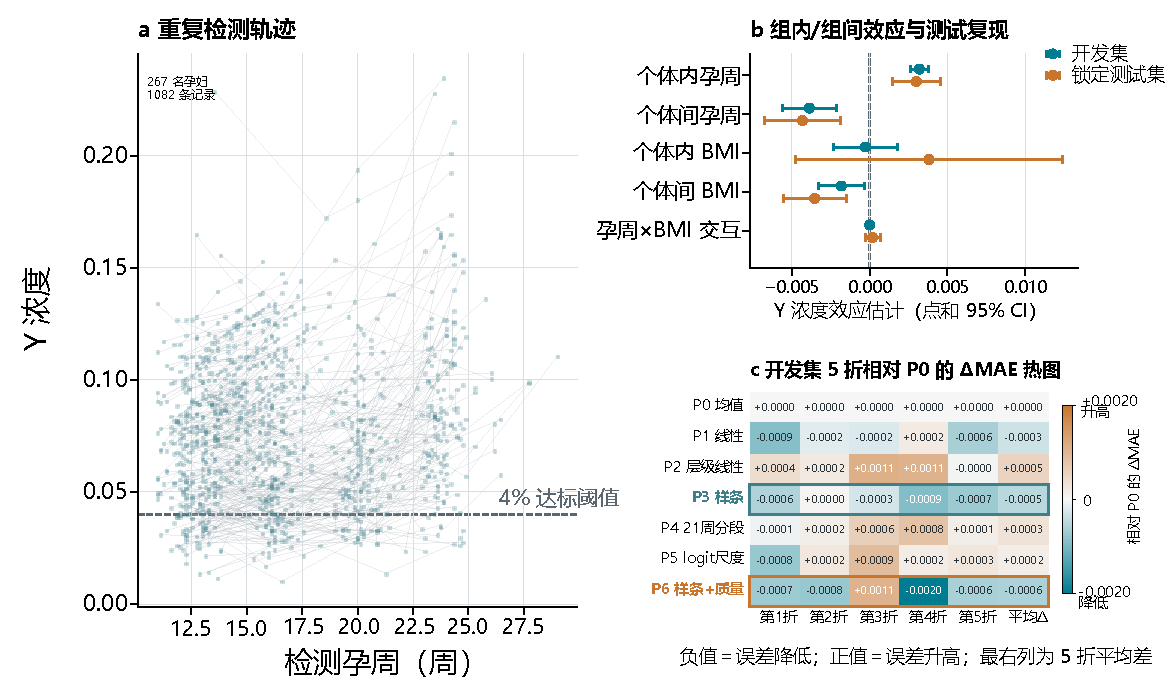
\includegraphics[width=\textwidth]{论文图表/q1_figure_1.pdf}
			\caption{问题1的个体轨迹、组内/组间效应及候选模型验证。a：Mundlak分解下的开发集估计与锁定测试集独立重估，点为效应估计值，横线为95\%置信区间；b：267名孕妇的1082条重复检测轨迹，虚线为Y浓度4\%达标阈值；c：开发集孕妇级5折验证中各候选模型相对P0均值模型的孕妇等权$\Delta$MAE热图，每格以同一折的P0误差为基准，负值表示误差降低、正值表示误差升高，最右列为5折平均差。}
			\label{fig:q1_structure_validation}
			\end{figure}

			模型冻结后，在53名锁定测试孕妇的214条记录上作一次外部评估。开发集和测试集的孕妇等权MAE分别为0.023423和0.023463，孕妇等权RMSE分别为0.025671和0.025745；三个可检验的核心方向（个体内孕周为正、个体间孕周为负、个体间BMI为负）在测试队列独立重估后保持一致。该检验支持关系方向的可复现性，但并不改变模型的解释性定位。
			
			\subsection{误差分析与方向转变}
			主模型在开发集和锁定测试集的记录级$R^2$分别为0.201和0.253，$R^2$确实很低，但这并非是由于线性形式选择错误造成的。在6.1节的预实验中，样条、21周分段、log/logit变换及质量扩展在孕妇级交叉验证中均未达到预设升级条件，最佳方案相对均值基线的MAE改善也只有2.28\%。这说明仅凭孕周、BMI及现有质量字段，未被解释的波动并非可由继续增加函数自由度稳定捕获。若为了提高样本内$R^2$继续堆叠变量或结点，只会把少量孕妇的轨迹和技术噪声拟合成表面规律。

			误差的首要来源是强烈且不可直接观测的个体基线差异。重复测量的ICC为0.658，说明同一孕妇的检测结果具有较强相关性，遗传背景、胎盘生物学状态和未记录的检测条件等因素会以个体基线差异的形式进入残差。这里需要区分“纳入随机性”与“解释个体差异”：预实验P2用随机截距将观测写成$y_{ij}=f(t_{ij},b_{ij})+u_i+\varepsilon_{ij}$，可以估计$u_i$的总体方差，识别重复测量的相关结构，并据此判断正式推断必须按孕妇聚类；但模型并未观测到决定$u_i$的具体因素，因而不能仅凭孕周、BMI和质量字段预先确定某名孕妇的基线。

			这一差别也再次验证了预实验的验证结果。对已有多次检测的孕妇，历史Y浓度可以帮助收缩估计其$u_i$，随机截距因而可能改善回顾性拟合；而孕妇级分组交叉验证要求验证折中的孕妇从未出现在训练折中。此时没有个人历史可供估计，只能取$\mathrm E(u_i)=0$，预测方差中仍保留$\mathrm{Var}(u_i)$。表\ref{tab:q1_pilot}中P2的孕妇等权MAE较P1恶化3.35\%。这个结果不表示个体随机性不存在，而是说明这种随机性虽能被量化，却尚不能由现有协变量转化为新孕妇的预测信息。

			第二类误差来自技术复测与质量信息的不完全可观测性。复测组中位数口径下核心效应方向未反转，说明技术复测并未制造主结论；但质量扩展相对无质量样条仅改善0.44\%，且bootstrap区间跨过零。低GC、读段关系冲突、比对率和过滤率等字段只能记录部分技术过程，不能替代未记录的平台批次、样本处理及生物学波动。因此，质量变量适合作为稳健性边界，而不足以支撑把残差解释为可消除的测量误差。

			第三个、也最容易导致错误叙述的来源是组内与组间效应的方向转变：同一孕妇随孕周增加时，$y$平均上升；但平均检测孕周更晚的孕妇群体，其平均$y$反而更低。后一个负系数不是“孕周越大Y浓度越低”的生物学结论，而是不同孕妇的BMI、首检时点、未观测个体基线及就诊路径共同混入横截面比较后的结果。若忽略式\eqref{eq:q1_mundlak_decompose}，把全部记录合并回归，便会把这种组间混杂错写成纵向规律。另有5条锁定测试记录的孕周或BMI落在开发集范围之外，故边界处的线性外推同样不应成为结论依据。

			因此，在误差分析后，真正的目标不是把每名孕妇的$y_{ij}$预测到很高精度，而是建立后续决策可用的结构约束：孕周具有可复现的个体内正向关联，BMI相关差异主要出现在孕妇之间，且个体重复检测不能当作独立证据。后续模型应把评价对象从连续浓度的$R^2$转为BMI分组下$Y\geq4\%$的达标概率、潜在风险和推荐时点的稳定性。
			
			\subsection{第一问结论}
			问题1给出的关系模型和显著性检验可以支持以下结论：
			\begin{enumerate}[leftmargin=2em,itemsep=2pt]
			\item 同一孕妇内，孕周每增加1周，Y浓度平均增加约0.003203，且该方向在锁定测试队列中得到复现；
			\item 孕妇间的平均BMI与Y浓度呈稳定负相关，但这一结果描述的是群体间差异；
			\item 重复测量相关性很强，后续分析必须以孕妇而非检测记录作为独立划分与不确定性评估单位；
			\item 现有证据不支持将21周设为统一转折点，也不支持把高自由度非线性、目标尺度变换或质量扩展升级为主模型。
			\end{enumerate}

			同时，以下推论必须禁止外推：不能将个体间BMI负相关解释为“孕期减重必然提高Y浓度”；不能将组间孕周负系数解释为个体内随孕周下降；不能据本模型为新孕妇报出高精度Y浓度或精确达标周；也不能把结论直接推广到开发集范围外的孕周、BMI、检测平台或地区。$R^2$约为0.2只说明固定协变量解释的记录级波动有限，并不否定经过聚类稳健推断后得到的关系方向；但它足以否定把该模型解释为个体预测器。

			据此分析，问题二接收的不是问题1的全样本拟合值，而是三项约束：一是以$Y\geq0.04$作为达标定义；二是按孕妇内检测序列构造左删失、区间删失和右删失的首次达标信息，不能把首次阳性当作真实达标时点；三是在BMI分组内比较达标概率与潜在风险，而非按单条浓度预测安排检测。
			
			\section{问题二建模}
			\subsection{任务解释与结论预览}
			\subsubsection{从“最早达标”到检测时点决策}
			问题二要求按BMI分组，并为每组选择使潜在风险尽量小的NIPT时点。这里有两个容易混淆的量：一是Y染色体浓度首次达到$4\%$的潜在时刻，二是在某一孕周实施检测后得到可靠结果的概率。附件中同一孕妇存在纵向复测和同次采血技术复测，且116名男胎孕妇出现相邻Y浓度下降，因此不能把第一条阳性记录直接当作真实首次达标时刻。本文把目标改写为：先估计孕周$t$时获得可靠检测结果的概率，再在检测失败、重检次数和延迟风险之间选择时点。

			开发集含214名孕妇。技术复测取同组中位数后，首次达标信息表现为174例左删失、35例区间删失和5例右删失；题面五组人数为5、108、83、15和3。这样的信息结构足以比较低容量策略，却不足以支持在两端小样本中自由搜索精细切点。本文因此先检验“BMI是否需要差异化检测安排”，检验通过才保留组间系数；否则仍按BMI报告风险，但不强行制造不同检测周。

			\subsubsection{题目要求与本文回答}
			表\ref{tab:q2_answer_preview}先给出第二问的答案。BMI$=30$和$35$只用于风险沟通，估计层由数据决定是否保留组间差异。孕妇级验证最终选择共用概率模型，所以三个粗分层得到相同策略；这是一项模型选择结果，不是预先假定。

			\begin{table}[H]
			\centering
			\footnotesize
			\renewcommand{\arraystretch}{1.18}
			\setlength{\tabcolsep}{3pt}
			\caption{问题二的任务、回答及证据对应关系}
			\label{tab:q2_answer_preview}
			\begin{tabularx}{\textwidth}{@{}p{0.16\textwidth}p{0.38\textwidth}X@{}}
			\toprule
			题目要求 & 本文回答 & 主要证据 \\
			\midrule
			BMI合理分组 & 采用$<30$、$[30,35)$、$\geq35$三个风险沟通层；估计层允许完全合并 & 四种数据分区均无稳定增益；500次选择bootstrap全部选择单组 \\
			每组最佳时点 & 三组采用同一检测--重检策略；基准情景首检为10.5周，全情景最优值为10--22.5周 & 共用系数模型通过one-SE规则；192个预设情景中136个可行 \\
			潜在风险最小 & 同时考虑期望检测次数、未获得可靠结果概率、延迟损失和错误接受概率 & 有限周网格的Pareto前沿与情景目标函数 \\
			检测误差影响 & 误差改变可行率和推荐周数，但没有产生可复现的BMI组间差异 & 1000次联合bootstrap；56/192个情景达到稳定标准 \\
			\bottomrule
			\end{tabularx}
			\end{table}

			问题二从上游数据处理到条件策略输出的两级计算流程见图\ref{fig:q2_method_flowchart}。

			\begin{figure}[H]
			\centering
			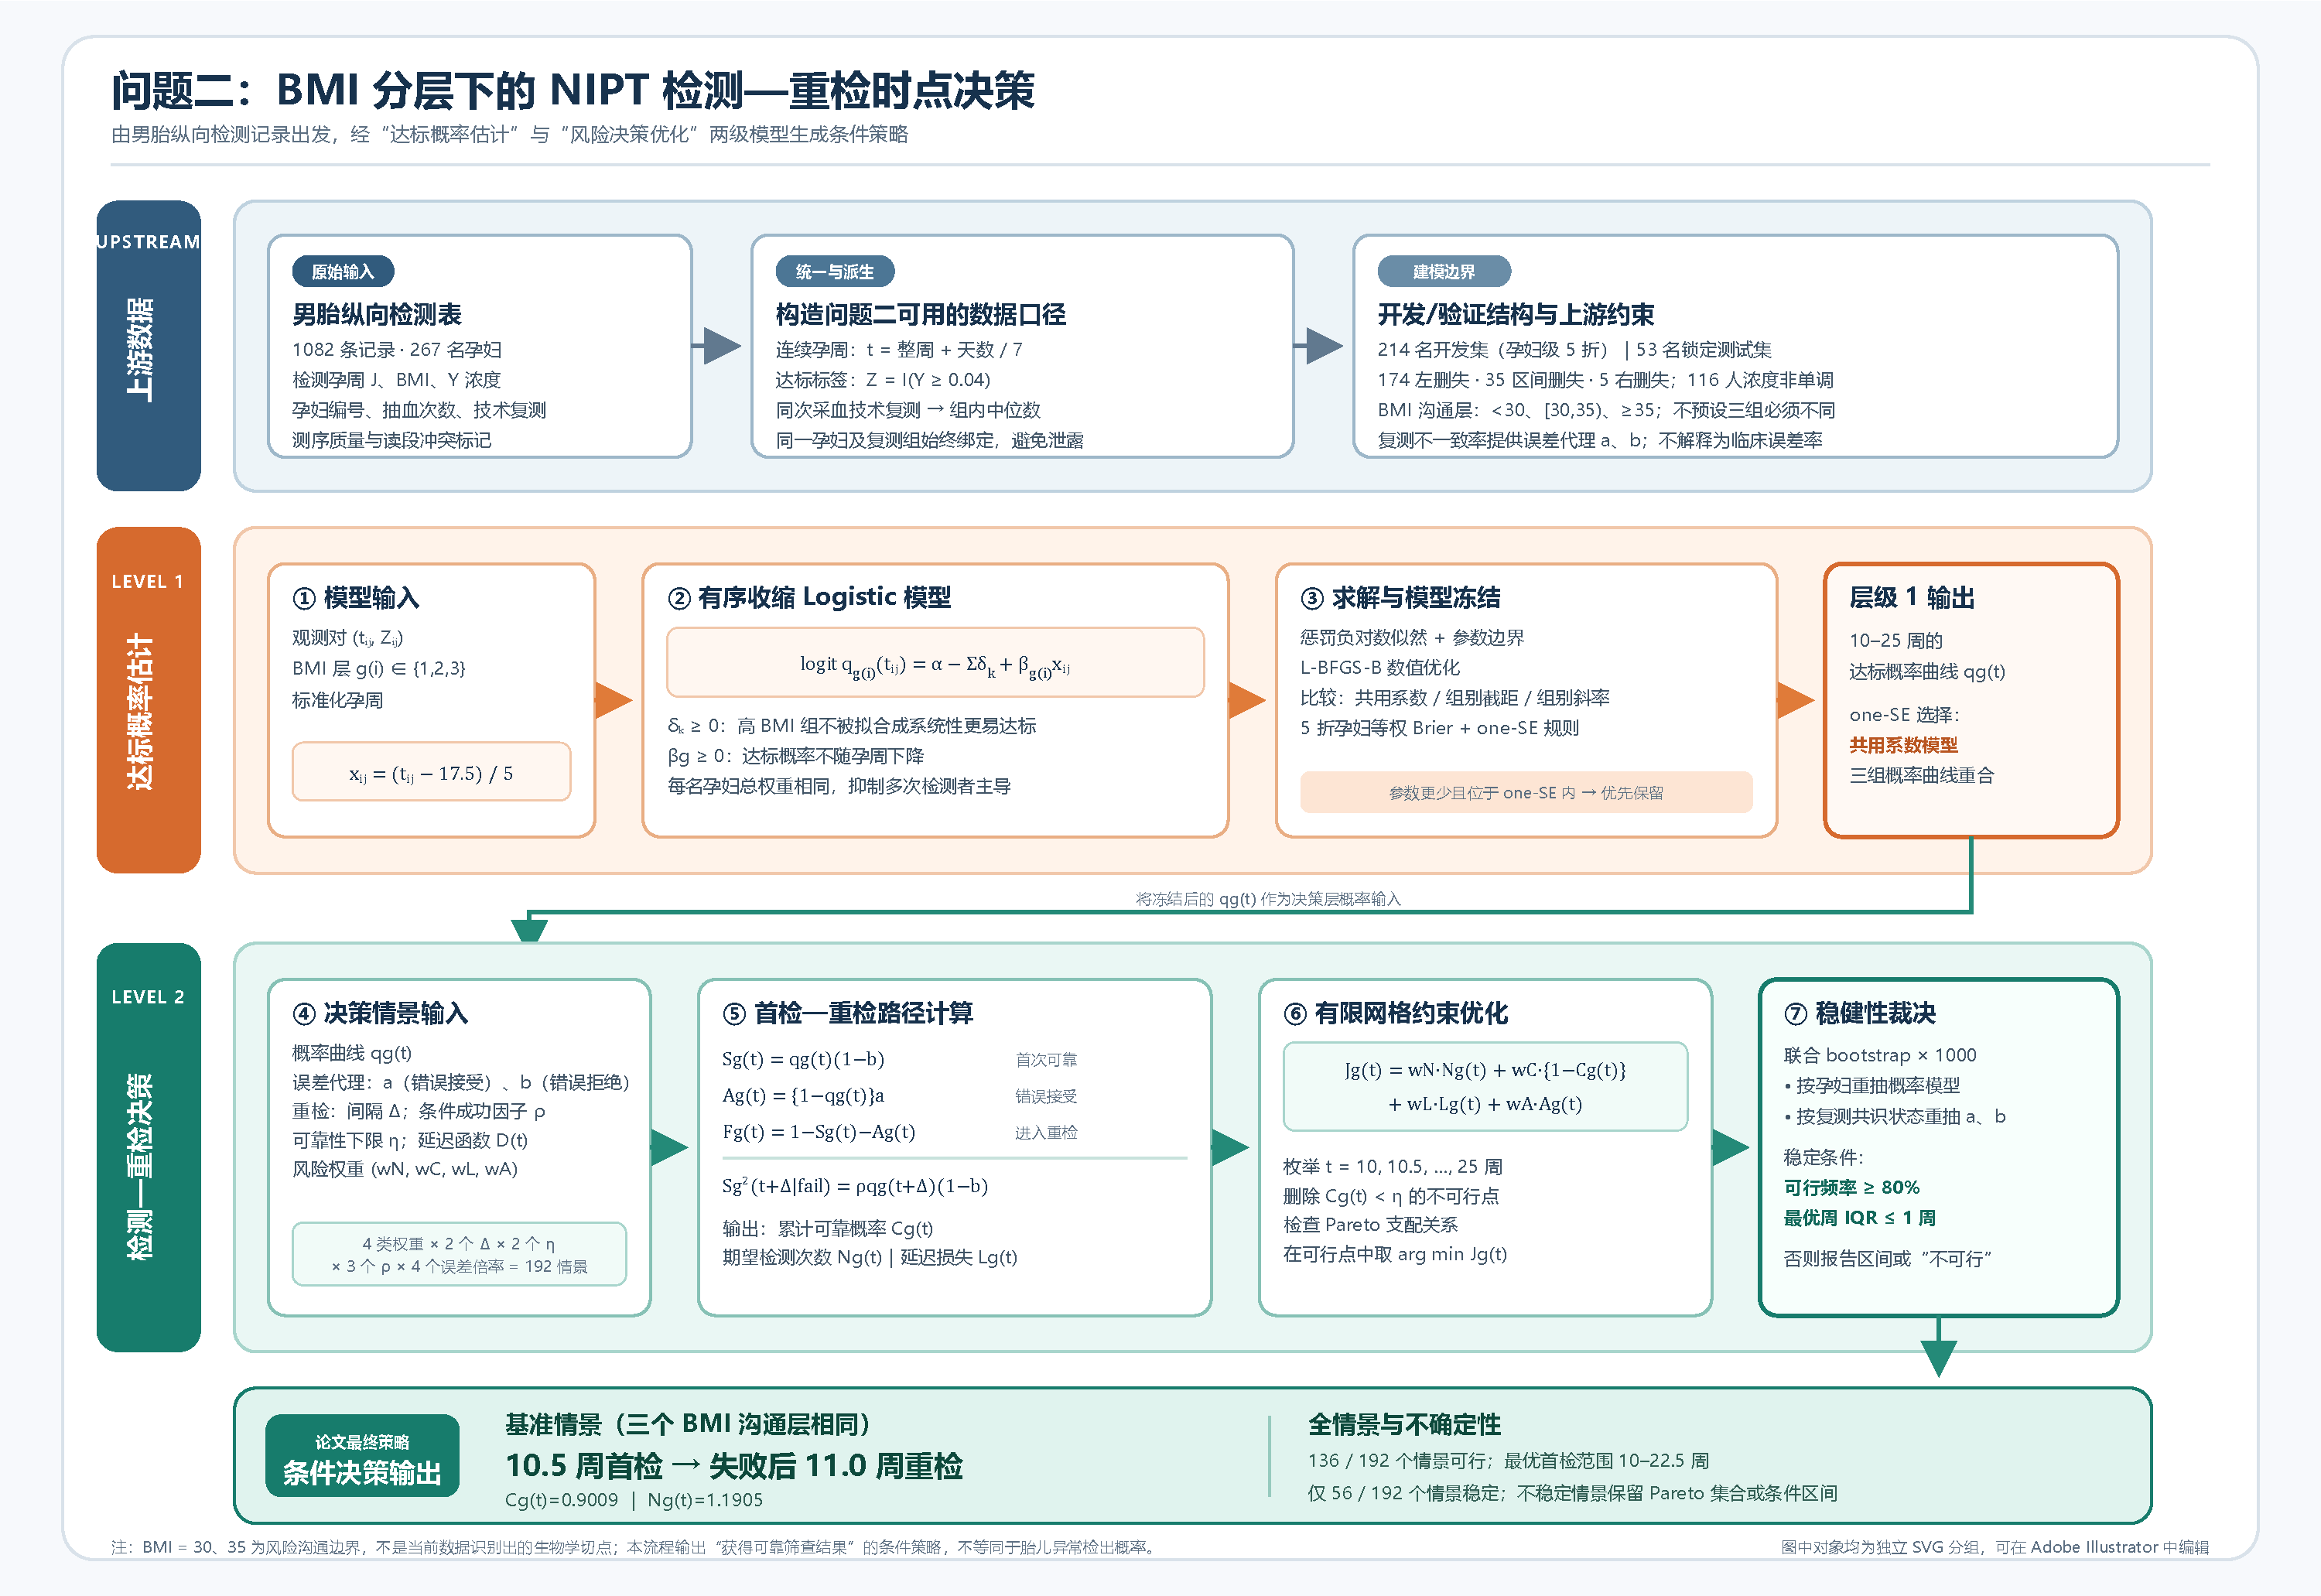
\includegraphics[width=\textwidth]{论文图表/q2_method_flowchart_vector.pdf}
			\caption{问题二的两级建模与计算流程。上游数据经统一口径和孕妇级验证后，先由估计层生成达标概率曲线，再由决策层计算首检--重检路径、执行约束风险优化并进行稳健性裁决。}
			\label{fig:q2_method_flowchart}
			\end{figure}

			\subsection{BMI差异化安排的必要性检验}
			\subsubsection{候选路线与预设判据}
			为避免看到结果后反复改切点，开发集内固定5折孕妇级划分，同一孕妇及其技术复测不跨折，锁定测试集不参与本节新增策略的选择。以仅孕周Logistic模型P0为基线，依次比较题面BMI五组、连续BMI低阶项、低自由度样条、区间删失Weibull AFT和连续Y浓度反演。主指标为孕妇等权Brier分数，同时检查对数损失、校准误差、折间胜出次数和阈值时点波动。

			判据在实验前固定：BMI候选相对P0的Brier改善至少达到$3\%$，才认为BMI提供了足以改变安排的增益；样条或反演路线相对其直接对照须改善$5\%$且至少4折胜出，才允许提高容量或改变拟合方向。表\ref{tab:q2_pilot}列出全部探针。最好的直接概率模型P1仅改善$1.60\%$，而最低Brier对应的P5相对P1只改善$0.02\%$。六条路线均未达到各自升级条件。

			\begin{table}[H]
			\centering
			\footnotesize
			\caption{差异化安排必要性检验的5折结果（214名开发集孕妇）}
			\label{tab:q2_pilot}
			\begin{tabularx}{\textwidth}{@{}cXcccc@{}}
			\toprule
			编号 & 模型结构 & Brier & 相对P0改善 & 胜出折数 & 最大时点SD/周 \\
			\midrule
			P0 & 仅孕周Logistic & 0.115946 & -- & -- & 1.70 \\
			P1 & 孕周+题面BMI五组 & 0.114095 & $1.60\%$ & 3/5 & 3.18 \\
			P2 & 连续BMI+交互项 & 0.114484 & $1.26\%$ & 4/5 & 3.15 \\
			P3 & 孕周与BMI低自由度样条 & 0.114304 & $1.42\%$ & 3/5 & 5.18 \\
			P4 & 区间删失Weibull AFT & 0.116791 & $-0.73\%$ & 2/5 & 1.24 \\
			P5 & 连续Y低阶回归后反演 & \textbf{0.114072} & $1.62\%$ & 4/5 & 2.46 \\
			\bottomrule
			\end{tabularx}
			\end{table}

			\subsubsection{有限切点比较与稳定性裁决}
			数据分区只比较$\varnothing$、$\{32\}$、$\{32,36\}$和题面切点$\{28,32,36,40\}$，分别对应不分组、两组、三组和五组。每个分区均拟合有序收缩Logistic模型，正则参数固定为
			\[
			\lambda\in\{0,10^{-4},10^{-3},10^{-2},10^{-1},1,10,100\},
			\]
			并使用one-SE规则。强收缩后，单组、两组、三组和五组的Brier分数依次为0.115981、0.115963、0.115916和0.115916，最大差仅$6.5\times10^{-5}$；500次孕妇bootstrap重新执行选择流程，单组被选中500次。因此，数据支持“当前样本不能识别稳定切点”，但不能推出BMI与Y浓度无关。

			\subsubsection{方向转变与文献依据}
			已有队列研究发现，胎儿游离DNA比例通常随孕周增加、随母体体重或BMI增加而下降，但等待的收益会随人群和检测平台变化\citeup{1,7}。统计方法研究指出，任意切分连续变量会损失信息，并使结论依赖边界\citeup{8,9}；首次无结果后的重抽成功率还与首次浓度、体重和采样间隔有关\citeup{10,13}。这些研究支持保留BMI风险分层，却不支持从本样本移植精确切点或检测周。

			基于上述证据，本文不再搜索新的BMI断点，而采用$<30$、$[30,35)$和$\geq35$三个外部可解释的粗分层。三个标签只承担风险汇总和结果沟通；概率模型仍比较共用系数、组别截距和组别斜率，若组别参数不能形成稳定增益，就收缩到同一曲线。决策对象也由“单次检测的精确达标周”转为“首次检测--失败重检”的条件策略。

			\begin{figure}[H]
			\centering
			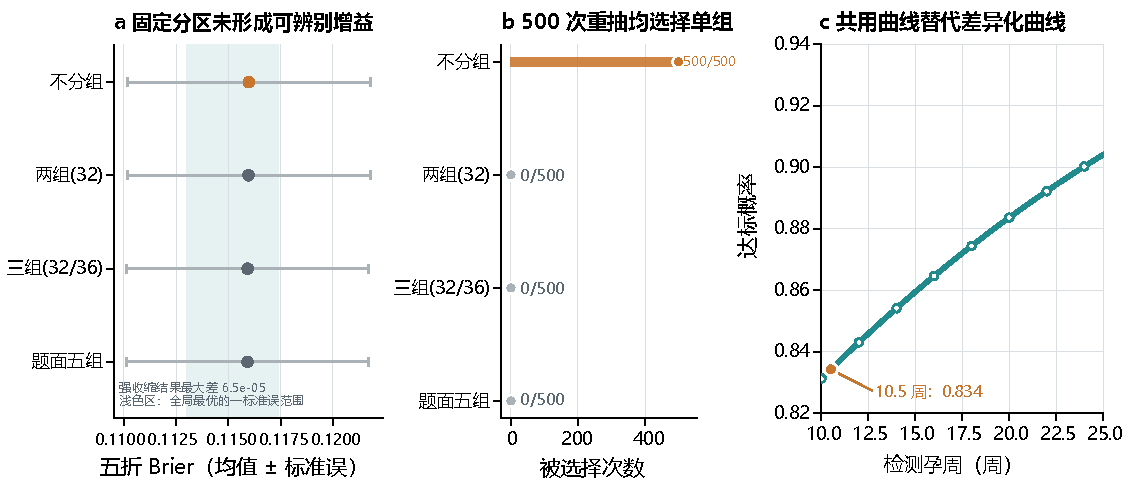
\includegraphics[width=\textwidth]{论文图表/q2_figure_1.pdf}
			\caption{BMI差异化检测安排的必要性检验。a：四种预设BMI分区在强收缩下的孕妇级五折Brier分数，点和横线分别为均值与标准误，浅色区域表示全局最优结果的一标准误范围；b：500次孕妇级选择bootstrap中各分区被选中的次数；c：one-SE规则选中的共用系数模型所给出的达标概率曲线，三个BMI粗分层的预测值完全重合，橙色点标出10.5周的达标概率。交叉验证与重抽选择共同表明，当前开发集不足以支持不同BMI组采用不同概率曲线；BMI分层仅用于风险沟通。}
			\label{fig:q2_route_evidence}
			\end{figure}

			\subsection{主模型建立与求解}
			\subsubsection{估计层：有序收缩达标概率模型}
			令$Z_{ij}=\mathbb{I}(y_{ij}\geq0.04)$，$g(i)\in\{1,2,3\}$为第$i$名孕妇的BMI粗分层，标准化孕周为$x_{ij}=(t_{ij}-17.5)/5$。用于比较组间差异的完整模型写为
			\begin{equation}
			\operatorname{logit}q_{g(i)}(t_{ij})
			=\alpha-\sum_{k=2}^{g(i)}\delta_k+\beta_{g(i)}x_{ij},
			\qquad \delta_k\geq0,\ \beta_g\geq0,
			\label{eq:q2_probability}
			\end{equation}
			其中$q_g(t)=P(Z=1\mid t,g)$。$\delta_k\geq0$保证更高BMI组不会被拟合成系统性更容易达标，$\beta_g\geq0$保证预测达标概率不随孕周下降。每名孕妇的全部记录总权重相同，以免检测次数多的孕妇主导估计。

			参数通过带边界的惩罚似然求解：
			\begin{equation}
			\begin{aligned}
			\mathcal{L}(\theta)=
			&-\sum_{i=1}^{n}\frac{1}{m_i}\sum_{j=1}^{m_i}
			\left[Z_{ij}\log q_{g(i)}(t_{ij})+(1-Z_{ij})\log\{1-q_{g(i)}(t_{ij})\}\right]\\
			&+\lambda_I\sum_{k=2}^{3}\delta_k^2
			+\lambda_S\sum_{g=1}^{3}(\beta_g-\bar\beta)^2,
			\end{aligned}
			\label{eq:q2_penalized_likelihood}
			\end{equation}
			其中$m_i$为第$i$名孕妇的有效观测数。本文比较共用系数、组别截距及组别截距加斜率三类配置；组别截距惩罚固定为$\lambda_I=100$，组别斜率的$\lambda_S$取$1,10,100$。各配置在相同的5折划分上计算Brier分数，落入全局最优值一个标准误以内时，优先选择参数更少的模型。式\eqref{eq:q2_penalized_likelihood}采用L-BFGS-B算法求解，概率在数值计算时截断至$[10^{-8},1-10^{-8}]$。

			\subsubsection{决策层：检测--重检路径与风险函数}
			估计层给出$q_g(t)$后，引入检测误差和至多一次重检。记$a$为真实未达标却被判为达标的概率代理，$b$为真实达标却被判为未达标的概率代理。首次获得可靠结果、错误接受和需要重检的概率分别为
			\begin{equation}
			S_g(t)=q_g(t)(1-b),\qquad
			A_g(t)=\{1-q_g(t)\}a,\qquad
			F_g(t)=1-S_g(t)-A_g(t).
			\label{eq:q2_first_path}
			\end{equation}
			若首次失败后间隔$\Delta$周重检，令$\rho\in\{0.50,0.75,1.00\}$表示条件二次成功因子，则
			\begin{equation}
			S_g^{(2)}(t+\Delta\mid\mathrm{fail})
			=\rho q_g(t+\Delta)(1-b).
			\label{eq:q2_second_success}
			\end{equation}
			这里$\rho$是情景参数，不是附件直接估计的临床重抽成功率。累计获得可靠结果的概率$C_g(t)$、期望检测次数$N_g(t)$和延迟损失$L_g(t)$定义为
			\begin{equation}
			\begin{aligned}
			C_g(t)&=S_g(t)+F_g(t)S_g^{(2)}(t+\Delta\mid\mathrm{fail}),\\
			N_g(t)&=1+F_g(t),\\
			L_g(t)&=D(t)+F_g(t)\{D(t+\Delta)-D(t)\},
			\end{aligned}
			\label{eq:q2_path_outputs}
			\end{equation}
			其中$D(t)$按题面规定保持早期低于中期、晚期高于中期的顺序，并在同一风险阶段内随孕周非减。$C_g(t)$只表示获得可靠筛查结果的概率，不能解释为胎儿异常检出率。

			对情景$\omega=(w_N,w_C,w_L,w_A,\Delta,\eta,\rho,a,b)$，在统一量纲后定义
			\begin{equation}
			J_g(t;\omega)=w_NN_g(t)+w_C\{1-C_g(t)\}
			+w_LL_g(t)+w_AA_g(t),
			\label{eq:q2_objective}
			\end{equation}
			并满足
			\begin{equation}
			t\in\{10,10.5,\ldots,25\},\qquad C_g(t)\geq\eta.
			\label{eq:q2_constraints}
			\end{equation}
			四类权重分别侧重均衡、可靠性、延迟和资源；$\Delta\in\{0.5,1.0\}$，$\eta\in\{0.90,0.95\}$，误差倍率取$0,0.5,1,1.5$。共形成$4\times2\times2\times3\times4=192$个预设情景。正文先报告$(N_g,1-C_g,L_g,A_g)$的Pareto非支配点，再给出各情景的最优时点和范围，避免用单一主观权重替代题目中没有提供的临床损失。

			\subsubsection{有限网格求解算法}
			模型只含有限周网格和有限情景，不需要启发式搜索。求解步骤如下：
			\begin{enumerate}[label=\arabic*),itemsep=0pt,topsep=2pt]
			\item 在固定5折上比较概率模型，以one-SE规则冻结共用或分组配置；
			\item 在全部214名开发集孕妇上重估入选模型，生成10--25周的$q_g(t)$；
			\item 对每个情景和每个候选周计算式\eqref{eq:q2_first_path}--\eqref{eq:q2_objective}，删除不满足式\eqref{eq:q2_constraints}的点；
			\item 对可行点逐一检查Pareto支配关系，并按$J_g(t;\omega)$选出情景最优值；若没有可行点，则记录“不可行”，不向边界外推；
			\item 以孕妇为单位重抽概率模型，并按技术复测组分层重抽误差率，共重复1000次。情景可行频率不低于$80\%$且最优周IQR不超过1周时，记为稳定。
			\end{enumerate}

			\subsection{求解结果}
			\subsubsection{组间系数的最终决定}
			表\ref{tab:q2_model_selection}给出固定$30/35$粗分层后的系数比较。组别截距模型取得最低平均Brier，但共用模型与其差值只有$4.2\times10^{-5}$，远小于5折标准误。按照one-SE规则，共用系数模型参数最少，故作为策略层的概率输入。三个BMI层随后的概率曲线和策略数值完全相同。

			\begin{table}[H]
			\centering
			\footnotesize
			\renewcommand{\arraystretch}{1.15}
			\caption{固定BMI粗分层后的概率模型比较}
			\label{tab:q2_model_selection}
			\begin{tabular}{lcccc}
			\toprule
			配置 & 平均Brier & 5折标准误 & 最差折Brier & one-SE内 \\
			\midrule
			组别截距 & \textbf{0.115939} & 0.005801 & 0.131109 & 是 \\
			组别截距+斜率（$\lambda_S=100$） & 0.115947 & 0.005803 & 0.131134 & 是 \\
			共用系数 & 0.115981 & 0.005824 & 0.131167 & 是，\textbf{入选} \\
			\bottomrule
			\end{tabular}
			\end{table}

			\subsubsection{基准情景与全情景结果}
			为给出可复核的代表结果，图形和主表采用预先指定的基准情景。其参数为
			\[
			(w_N,w_C,w_L,w_A)=(0.20,0.35,0.25,0.20),\quad
			\Delta=0.5,\quad \eta=0.90,\quad \rho=0.75,
			\]
			误差倍率取1。三个BMI层的最优首检周均为10.5周，失败后于11.0周重检；累计可靠结果概率为0.9009，期望检测次数为1.1905。表\ref{tab:q2_strategy_answer}中的10.5周是基准情景解，不是脱离参数条件的临床常数。

			\begin{table}[H]
			\centering
			\footnotesize
			\renewcommand{\arraystretch}{1.16}
			\caption{问题二的BMI分组与检测--重检策略结果}
			\label{tab:q2_strategy_answer}
			\begin{tabular}{lcccccc}
			\toprule
			BMI区间 & 首检/周 & 重检/周 & $C_g(t)$ & $N_g(t)$ & 全情景范围/周 & 可行率 \\
			\midrule
			$<30$ & 10.5 & 11.0 & 0.9009 & 1.1905 & 10--22.5 & $70.8\%$ \\
			$[30,35)$ & 10.5 & 11.0 & 0.9009 & 1.1905 & 10--22.5 & $70.8\%$ \\
			$\geq35$ & 10.5 & 11.0 & 0.9009 & 1.1905 & 10--22.5 & $70.8\%$ \\
			\bottomrule
			\end{tabular}
			\end{table}

			192个情景中有136个至少存在一个可行时点。可行情景最优首检周的下四分位数、中位数和上四分位数分别为10、10和15周，最大值为22.5周。三组结果相同，说明当前数据没有给出仅凭BMI推迟高BMI孕妇首次检测的依据。高可靠性或悲观重检假设导致不可行时，模型输出“不可行”或条件区间，而不把25周边界当作推荐值。

			\begin{figure}[H]
			\centering
			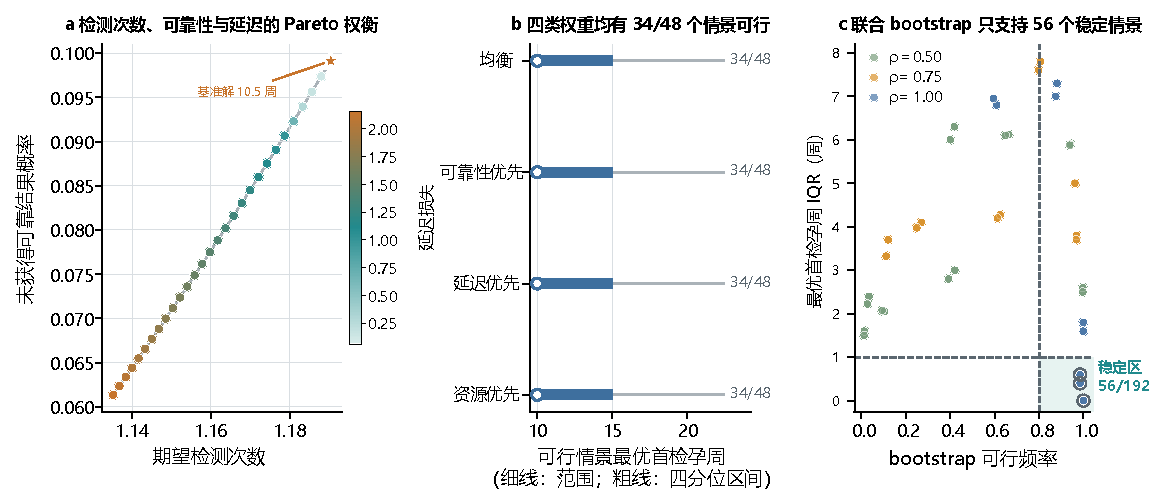
\includegraphics[width=\textwidth]{论文图表/q2_figure_2.pdf}
			\caption{检测次数、可靠性与延迟之间的权衡及其稳健性。a：基准情景中29个可行时点的Pareto权衡，横轴为期望检测次数，纵轴为未获得可靠结果概率，颜色表示延迟损失，星号为10.5周基准解；b：四类权重下可行情景最优首检孕周的范围与四分位区间，每类34/48个情景可行；c：192个预设情景的1000次联合bootstrap结果，虚线表示可行频率不低于80\%且最优周IQR不超过1周的稳定标准，空心外圈标出56个稳定情景。情景范围描述外生决策假设的变化，不是抽样置信区间。}
			\label{fig:q2_strategy_robustness}
			\end{figure}

			\subsection{检测误差与稳健性检验}
			\subsubsection{误差口径与参数扰动}
			同次采血技术复测组没有临床真值，故本文以复测组中位数形成共识标签，再计算单条复测相对该共识的阈值不一致率。点估计的假阳性代理为0.1304，假阴性代理为0.0556。二者只用于误差情景，不能表述为NIPT的临床假阳性率和假阴性率。联合bootstrap按孕妇重抽概率模型，并按共识状态分层重抽30个技术复测组；1000次重复中，假阳性代理的$2.5\%$、中位数和$97.5\%$分位数为0、0.1304和0.2500，假阴性代理对应为0、0.0545和0.1200。

			\subsubsection{网格、重检假设与联合bootstrap}
			表\ref{tab:q2_robustness}汇总三项决定性检验。首先，将主网格由0.5周细化至0.1周后，136个共同可行情景的最优时点中位绝对差为0，最大差0.4周，说明数值网格足够细。其次，$\rho$由0.50增至1.00时，可行率由$37.5\%$升至$100\%$，二次成功假设会实质改变策略。最后，仅56个情景同时达到可行频率和时点IQR标准，占$29.2\%$。因此，算法求解稳定不等于决策对外生参数稳定。

			\begin{table}[H]
			\centering
			\footnotesize
			\renewcommand{\arraystretch}{1.16}
			\caption{问题二的误差与稳健性检验结果}
			\label{tab:q2_robustness}
			\begin{tabularx}{\textwidth}{@{}p{0.25\textwidth}p{0.27\textwidth}X@{}}
			\toprule
			检验对象 & 结果 & 对题目回答的影响 \\
			\midrule
			0.5周与0.1周网格 & 中位绝对差0周；最大差0.4周；可行性无错配 & 排除离散网格过粗造成的时点漂移 \\
			二次成功因子$\rho$ & $0.50/0.75/1.00$时可行率为$37.5\%/75.0\%/100\%$ & 重检信息不足时必须报告情景范围，不能给无条件单点 \\
			1000次联合bootstrap & 56/192个情景稳定，稳定率$29.2\%$ & 只对稳定情景给点值，其余报告区间或不可行 \\
			误差率重抽 & 假阳性代理中位0.1304，假阴性代理中位0.0545 & 误差扩大可行性不确定性，但未产生BMI组间差异 \\
			\bottomrule
			\end{tabularx}
			\end{table}

			\subsection{第二问结论}
			第二问得到以下结论。
			\begin{enumerate}[label=\arabic*),itemsep=0pt,topsep=2pt]
			\item BMI按$<30$、$[30,35)$和$\geq35$分为三个风险沟通层。数据驱动的四种分区均未通过预设增益标准，500次选择bootstrap全部选择单组；固定粗分层后的one-SE比较也选中共用系数模型。因此，现有样本不支持三组采用不同检测时点。
			\item 在均衡权重、可靠性下限0.90、二次成功因子0.75、误差倍率1和0.5周重检间隔的基准情景下，三个BMI层均在10.5周首次检测，失败后于11.0周重检，累计可靠结果概率为0.9009。该时点只对基准情景成立。
			\item 192个预设情景中136个可行，可行情景的最优首检周为10--22.5周。1000次联合bootstrap仅有56个情景达到稳定标准，说明检测误差、可靠性要求和条件重检成功率决定了可否给出单点。对不稳定或不可行情景，本文保留Pareto集合和条件区间，不作边界外推。
			\item 本模型给出“获得可靠NIPT结果”的条件策略，不估计胎儿异常检出率。附件缺少临床损失和完整重抽结局，故$\rho$与误差率只作情景参数。
			\end{enumerate}

			\section{问题三建模}
			\subsection{模型建立与求解}
			\subsubsection{题意转化与模型复用}
			问题三要求在BMI之外考虑身高、体重、年龄等因素，并判断这些信息是否会改变分组和检测时点。附件中的“达标时间”并非精确观测的事件时间：同一孕妇的检测次数有限，Y染色体浓度还可能随技术误差出现非单调变化。本文仍以孕周$t$时Y染色体浓度达到$4\%$的概率$q_i(t)$描述达标过程，再由概率曲线和检测误差计算检测--重检路径的期望损失。这样既保留了题目中的“达标比例”，也避免把首次观测到达标的周数当成真实达标时刻。

			问题二已经固定了孕妇级数据划分、BMI风险沟通层、达标概率基线、检测--重检风险函数和192个参数情景。第三问沿用这些对象，使新增因素与问题二在同一批孕妇、同一折划分和同一损失函数下比较。复用部分只充当冻结基线；本问新增了字段可得性审计、体型共线性处理、多因素增量检验、非线性对照、失败后重检模型和策略回放。若某个因素只改善拟合、却不能稳定改变风险或时点，则不进入最终策略。

			\subsubsection{新增因素的概率模型}
			令$Z_{ij}=\mathbb{I}(y_{ij}\geq0.04)$，标准化孕周$x_{ij}=(t_{ij}-17.5)/5$。以问题二的共用系数模型为基线，检测前多因素候选写为
			\begin{equation}
			\operatorname{logit}q_i(t_{ij})
			=\alpha+\beta x_{ij}+\boldsymbol{\gamma}^{\mathsf T}\boldsymbol{u}_i,
			\label{eq:q3_multifactor_probability}
			\end{equation}
			其中$\boldsymbol{u}_i$从年龄、体型表达、受孕方式、怀孕次数和生产次数中选取。BMI满足$BMI=W/H^2$；本数据中该恒等式的最大计算误差为0，BMI、身高和体重同时入模时的VIF为97.503--317.581。因此体型部分只比较$BMI$、$BMI+$身高及身高$+$体重，不设置三者同时入模的候选。

			首检后的信息另建通道。对首次未获得可靠结果的孕妇，令$r_i$表示下一次检测可靠达标的条件概率，考察
			\begin{equation}
			\operatorname{logit}r_i
			=\theta_0+\theta_t t_i+\theta_{\Delta}\Delta_i+\theta_B BMI_i
			+\theta_d d_i+\boldsymbol{\theta}_Q^{\mathsf T}\boldsymbol{Q}_i,
			\label{eq:q3_retest_probability}
			\end{equation}
			其中$d_i$为首次Y浓度到$4\%$阈值的距离，$\boldsymbol{Q}_i$包括读段数、比对率、重复率、GC含量和过滤比例。式\eqref{eq:q3_retest_probability}只用于首检失败后的重检判断，不反向用于安排第一次检测。

			开发集含214名孕妇、821个技术复测中位数观测。全部候选使用相同的孕妇级五折划分，各孕妇等权。检测前候选须同时满足：折外Brier相对改善不少于$3\%$、至少4/5折优于基线、最差折恶化不超过$5\%$；固定非线性候选的改善门槛为$5\%$。这组规则在计算前确定，用来约束变量筛选和模型复杂度。

			\subsubsection{概率模型与风险函数的衔接}
			设$a$、$b$分别为错误接受和错误拒绝概率代理，$\Delta$为重检间隔，$\rho$为条件二次成功因子。由$q_g(t)$得到首次可靠、错误接受和首次失败概率
			\begin{equation}
			S_g(t)=q_g(t)(1-b),\quad
			A_g(t)=\{1-q_g(t)\}a,\quad
			F_g(t)=1-S_g(t)-A_g(t).
			\label{eq:q3_first_path}
			\end{equation}
			考虑至多一次重检后，累计可靠概率、期望检测次数和延迟损失为
			\begin{equation}
			\begin{aligned}
			C_g(t)&=S_g(t)+F_g(t)\rho q_g(t+\Delta)(1-b),\\
			N_g(t)&=1+F_g(t),\\
			L_g(t)&=D(t)+F_g(t)\{D(t+\Delta)-D(t)\},
			\end{aligned}
			\label{eq:q3_path_outputs}
			\end{equation}
			其中$D(t)$沿用问题二按早期、中期风险递增设置的延迟损失。将权重、重检间隔、可靠性下限、二次成功因子和误差参数记为
			\[
			\omega=(w_N,w_C,w_L,w_A,\Delta,\eta,\rho,a,b).
			\]
			对每个情景$\omega$，综合决策风险定义为
			\begin{equation}
			\min_{t\in\{10,10.5,\ldots,25\}}
			J_g(t;\omega)=w_NN_g(t)+w_C\{1-C_g(t)\}
			+w_LL_g(t)+w_AA_g(t),
			\quad C_g(t)\geq\eta.
			\label{eq:q3_risk_objective}
			\end{equation}
			四项依次对应检测资源、未获可靠结果、延迟发现和错误接受。本文不把$J_g$解释为临床不良结局概率；它是给定权重和误差情景下的无量纲决策损失。求解时先冻结通过筛选的概率模型，再把其概率曲线代入式\eqref{eq:q3_first_path}--\eqref{eq:q3_risk_objective}，逐场景枚举可行周并选取最小风险。

			\subsection{模型建立与求解结果}
			\subsubsection{多因素升级的筛选结果}
			表\ref{tab:q3_factor_results}给出新增因素相对问题二基线的折外结果。身高$+$体重是检测前表现最好的候选，Brier由0.115970降至0.113581，相对改善$2.06\%$，但只在3/5折胜出，没有达到预设标准。单独加入BMI改善$1.20\%$；年龄和怀孕次数分别使Brier恶化$0.92\%$和$0.84\%$。固定非线性模型相对低容量基线只改善$0.15\%$。这些结果没有支持检测前模型增加变量或容量。

			\begin{table}[H]
			\centering
			\footnotesize
			\renewcommand{\arraystretch}{1.15}
			\caption{新增因素相对问题二基线的折外比较}
			\label{tab:q3_factor_results}
			\begin{tabularx}{\textwidth}{@{}p{0.25\textwidth}cccX@{}}
			\toprule
			候选模型 & Brier & 相对改善 & 胜出折数 & 处置 \\
			\midrule
			问题二共用系数基线 & 0.115970 & -- & -- & 保留为比较基准 \\
			孕周$+$BMI & 0.114580 & $1.20\%$ & 4/5 & 未达$3\%$改善线 \\
			孕周$+$身高$+$体重 & \textbf{0.113581} & \textbf{$2.06\%$} & 3/5 & 改善不足，折间方向不稳 \\
			孕周$+$年龄 & 0.117035 & $-0.92\%$ & 0/5 & 不保留 \\
			固定非线性模型 & 0.115792 & $0.15\%$ & 2/5 & 不升级模型容量 \\
			条件重检质量模型 & 0.175768 & $17.08\%$ & 4/5 & 最差折恶化$28.48\%$，仅作辅助分析 \\
			\bottomrule
			\end{tabularx}
			\end{table}

			条件重检模型使用60名孕妇的97对“首次失败--后续检测”记录。加入阈值距离和测序质量后，Brier从0.211978降至0.175768，平均改善$17.08\%$；但五折标准差为0.130629，最差折恶化$28.48\%$。平均结果与最差折给出相反判断，现有样本不足以冻结新的重检模型。

			\subsubsection{最终概率模型与BMI分组策略}
			没有新增变量通过筛选后，最终模型收缩为问题二的共用系数模型：
			\begin{equation}
			\operatorname{logit}q_g(t)
			=1.919143+0.216430\frac{t-17.5}{5},
			\qquad g=1,2,3.
			\label{eq:q3_final_probability}
			\end{equation}
			三个$g$分别对应$BMI<30$、$30\leq BMI<35$和$BMI\geq35$。这些区间用于风险沟通，不是本数据识别出的生物学切点；式\eqref{eq:q3_final_probability}在三组中完全相同。第三问由此得到一个有约束的负结果：新增因素已经进入比较，但没有稳定证据支持据此另设BMI切点或调整首检周。

			基准情景取$(w_N,w_C,w_L,w_A)=(0.20,0.35,0.25,0.20)$、$\Delta=0.5$、$\eta=0.90$、$\rho=0.75$，误差倍率为1。表\ref{tab:q3_strategy_results}显示，三组均在10.5周首检，失败后于11.0周重检。10.5周的直接达标比例$q_g(t)$为0.8343；加入一次条件重检后，累计可靠概率为0.9009，总风险为0.2920。

			\begin{table}[H]
			\centering
			\footnotesize
			\renewcommand{\arraystretch}{1.15}
			\caption{基准情景下的BMI分组、检测时点与风险结果}
			\label{tab:q3_strategy_results}
			\begin{tabular}{lccccccc}
			\toprule
			BMI区间 & 首检/重检周 & $q_g(t)$ & $C_g(t)$ & $N_g(t)$ & $L_g(t)$ & $A_g(t)$ & $J_g(t)$ \\
			\midrule
			$<30$ & 10.5/11.0 & 0.8343 & 0.9009 & 1.1905 & 0.0595 & 0.0216 & 0.2920 \\
			$[30,35)$ & 10.5/11.0 & 0.8343 & 0.9009 & 1.1905 & 0.0595 & 0.0216 & 0.2920 \\
			$\geq35$ & 10.5/11.0 & 0.8343 & 0.9009 & 1.1905 & 0.0595 & 0.0216 & 0.2920 \\
			\bottomrule
			\end{tabular}
			\end{table}

			对192个情景和3个BMI层逐项回放后，第三问与冻结的问题二策略在576组比较中的最优周、重检周、累计可靠概率、风险分量和总风险差值均为0，Pareto时点集合的Jaccard系数为1。这个结果说明，当前多因素证据没有转化为可执行的时点变化，而不是说明身高、体重或年龄在其他人群中没有作用。

			\begin{figure}[H]
			\centering
			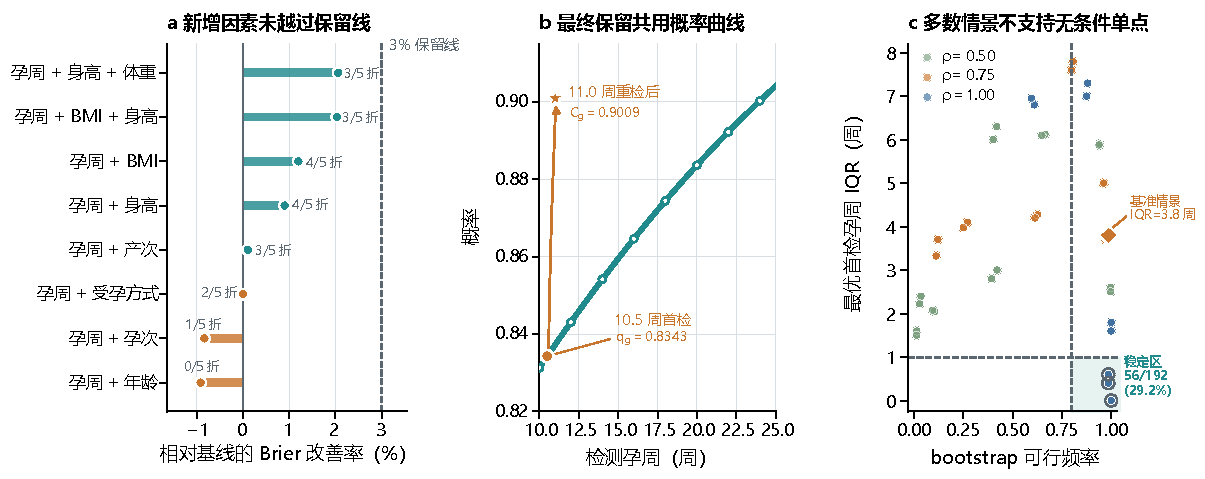
\includegraphics[width=\textwidth]{论文图表/q3_figure_1.pdf}
			\caption{第三问的因素筛选、共同策略与稳定性。a：214名开发集孕妇的固定五折验证中，检测前候选相对孕周基线的Brier改善率，标注为优于同折基线的折数，虚线为$3\%$预设保留线；b：最终模型中三个BMI报告层完全重合的达标概率曲线，圆点标出10.5周的直接达标概率，星号标出失败后于11.0周重检的累计可靠概率；c：192个预设情景各1000次联合bootstrap的可行频率与最优首检孕周IQR，虚线围成预设稳定区，空心外圈标出56个稳定情景，菱形为基准情景。三幅面板分别回答是否升级模型、是否采用差异化时点以及条件解能否外推。}
			\label{fig:q3_core_findings}
			\end{figure}

			\subsection{误差分析与稳健性检验}
			同次采血的技术复测没有临床真值。本文以复测组中位数形成共识标签，得到错误接受和错误拒绝概率代理；1000次分层bootstrap中，二者的中位数分别为0.1304和0.0545，对应的$95\%$分位区间为$[0,0.2500]$和$[0,0.1200]$。这些数值只描述附件内部的阈值不一致，不能当作NIPT的临床假阳性率和假阴性率。

			表\ref{tab:q3_robustness}汇总对最终回答影响最大的检查。0.5周网格细化至0.1周后，共同可行情景的最优时点中位绝对差为0，最大差0.4周，说明离散求解误差较小。二次成功因子$\rho$从0.50增至1.00时，场景可行率由$37.5\%$升至$100\%$，重检假设仍是主要不确定来源。192个情景中136个存在可行解，最优首检周覆盖10--22.5周；只有56个情景同时满足bootstrap可行频率不低于$80\%$且时点IQR不超过1周。

			\begin{table}[H]
			\centering
			\footnotesize
			\renewcommand{\arraystretch}{1.15}
			\caption{第三问的误差与稳健性检验}
			\label{tab:q3_robustness}
			\begin{tabularx}{\textwidth}{@{}p{0.25\textwidth}p{0.28\textwidth}X@{}}
			\toprule
			检验对象 & 结果 & 对第三问结论的影响 \\
			\midrule
			检测误差重抽 & $a$中位0.1304，$b$中位0.0545 & 误差改变可行性，但没有产生BMI组间差异 \\
			0.5周与0.1周网格 & 中位绝对差0周，最大差0.4周 & 基准时点不是由粗网格造成的数值假象 \\
			二次成功因子$\rho$ & 可行率$37.5\%/75.0\%/100\%$ & 重检信息不足时应报告条件区间 \\
			1000次联合bootstrap & 56/192个情景稳定，稳定率$29.2\%$ & 多数情景不支持无条件单点 \\
			基准情景 & 可行频率0.969，时点IQR为3.8周 & 10.5周是条件解，不是稳定的普遍推荐 \\
			策略等价检查 & 576/576组风险和时点差值为0 & 新增因素没有改变当前可执行策略 \\
			\bottomrule
			\end{tabularx}
			\end{table}

			\subsection{第三问结论}
			第三问在问题二概率--风险框架上加入了年龄、体型、受孕方式和孕产史，并把首次结果与测序质量单独用于失败后的重检建模。检测前表现最好的多因素候选仅改善Brier分数$2.06\%$，未越过预设保留线；重检质量模型的平均改善较大，但最差折恶化$28.48\%$。现有样本没有给出足以改变首检安排的稳定增量信息，最终模型因此保留共用系数形式，三个BMI报告层采用相同概率曲线。

			在基准风险情景下，条件最优方案为10.5周首检、11.0周重检，直接达标比例为0.8343，累计可靠概率为0.9009。该方案的bootstrap时点IQR为3.8周，且只有$29.2\%$的预设情景达到稳定标准。因此，10.5周只表示给定可靠性、误差、重检成功率和风险权重后的条件解。对其余情景，本文保留10--22.5周的可行范围或报告不可行，不给出脱离参数条件的统一临床时点。

			\section{问题四建模}
			\subsection{建模准备}
			\subsubsection{问题目标与文献综述}
			问题四要求利用女胎检测记录判断是否存在染色体异常。本文以AB列非空构造任一异常标签$y_i\in\{0,1\}$，并保留T13、T18、T21及其组合信息。模型需要对一条新的检测记录给出异常概率和判定依据，而不是把同一孕妇全部记录合并成一个终身标签。数据中44名曾出现异常记录的孕妇有43名同时存在正常记录，32个同次复测组中也有5组标签不一致。这种结构说明，AB更适合作为单次筛查结果，不能在没有核型金标准的情况下解释为临床确诊\citeup{4,12}。

			母体血浆cfDNA的相对染色体计数为非整倍体筛查提供了直接信号，早期研究据此识别T13、T18和T21异常\citeup{17,18}。GC偏倚会影响染色体读段统计，校正后可改善部分染色体任务的判别\citeup{14}。因此，问题四首先考察13、18、21号染色体Z值，再检验X染色体汇总量、GC和测序质量能否提供稳定增量。WISECONDOR依赖基因组窗口级读段，SeqFF需要常染色体区域计数及相应训练信息\citeup{19,20}；附件只给出汇总字段，不能复现这两类方法。本文据此把候选范围收缩为简单Z值规则、低容量逻辑回归和一个固定容量的非线性对照，并按STARD和TRIPOD的报告原则保留受试者流、阈值来源、判别与校准信息\citeup{15,16}。

			\subsubsection{预实验目标与设计}
			预实验主要解决三个会改变建模方向的问题。第一，同一孕妇有纵向检测和技术复测，若按记录随机划分，模型会在训练集和验证集中看到同一人的信息。第二，开发集中异常记录占比较低，准确率容易被全预测正常的结果掩盖。第三，题目列出的变量较多，但样本只包含147名孕妇；把全部字段直接交给复杂模型，可能得到较高的训练性能而无法泛化。

			为隔离这些风险，本文以孕妇为单位将147人分为110人的开发集和37人的锁定测试集。开发集含447条记录，其中54条为异常；内部使用固定五折孕妇级分组验证，锁定测试集在预实验中不读取特征和性能。主指标采用折外预测汇总后的PR-AUC，辅助考察异常召回率、特异度、balanced accuracy、Brier分数、最差折和训练--验证差距。所有预处理、正则参数和判定阈值均在训练折内确定。

			低容量候选采用带$L_2$正则的逻辑回归。令$\boldsymbol{x}_i$为第$i$条记录的标准化特征，模型表达式为
			\begin{equation}
			p_i=\Pr(y_i=1\mid\boldsymbol{x}_i)
			=\operatorname{logit}^{-1}\!\left(\beta_0+\boldsymbol{\beta}^{\mathsf T}\boldsymbol{x}_i\right),
			\label{eq:q4_pilot_logistic}
			\end{equation}
			并按固定顺序构造三个嵌套规格：M0仅含$Z_{13},Z_{18},Z_{21}$；M1加入$Z_X$和X染色体浓度；M2再加入总体及13、18、21号染色体GC含量。另设置全预测正常、单Z值规则和固定浅层随机森林作为对照。新增特征块的PR-AUC增益须达到0.03，并在至少4/5折同向；非线性模型还须比最佳低容量候选提高0.05，且不能越过最差折和泛化差距限制。预实验同时比较记录等权、孕妇等权和同次复测概率中位数三种口径，并检查质量尾部以及各亚型的折内事件数。

			\subsubsection{预实验结果与分析}
			开发集的折外结果见表\ref{tab:q4_pilot_results}。全预测正常和单Z值规则的PR-AUC分别为0.120805和0.130159；M0也只有0.141768。单靠13、18、21号染色体Z值不足以复现附件中的AB判定。加入X特征后，M1的PR-AUC升至0.466804；M2进一步达到0.537504，并取得0.611111的异常召回率和0.870229的特异度。GC块相对M1增加0.070700，且4/5折同向，因而M2成为预实验胜出候选。

			\begin{table}[H]
			\centering
			\footnotesize
			\renewcommand{\arraystretch}{1.15}
			\caption{问题四开发集固定五折OOF预实验结果}
			\label{tab:q4_pilot_results}
			\begin{tabularx}{\textwidth}{@{}p{0.15\textwidth}p{0.24\textwidth}ccccX@{}}
			\toprule
			候选 & 输入或规则 & PR-AUC & 召回率 & 特异度 & Brier & 预实验处置 \\
			\midrule
			全预测正常 & 概率恒为0 & 0.120805 & 0 & 1.000000 & 0.120805 & 平凡基线 \\
			最佳单Z规则 & $|Z_{13}|$内部学习阈值 & 0.130159 & 0.981481 & 0.061069 & -- & 判别力不足 \\
			M0 & $Z_{13},Z_{18},Z_{21}$ & 0.141768 & 0.666667 & 0.465649 & 0.251043 & 保留为回退基线 \\
			M1 & M0$+$X特征块 & 0.466804 & 0.685185 & 0.788804 & 0.184255 & 增益明显，稳定性待复核 \\
			\textbf{M2} & M1$+$GC特征块 & \textbf{0.537504} & 0.611111 & 0.870229 & 0.165042 & 预实验胜出候选 \\
			浅层随机森林 & 固定深度3、300棵树 & 0.446579 & 0.722222 & 0.809160 & 0.154986 & 不晋级 \\
			\bottomrule
			\end{tabularx}
			\end{table}

			尽管M2胜出,但并不等于确定采用。M1虽带来较大增益，但其训练--验证差距相对M0扩大0.078700，超过预设的0.05限制；M2仍受这一问题牵连。浅层随机森林的PR-AUC比M2低0.090925，仅1/5折优于低容量候选，平均训练--验证差距为0.347455，复杂模型路线因此被否决。三种重复测量口径的PR-AUC分别为0.537504、0.580503和0.558428，范围为0.042999，未越过0.05的路线改变线，说明按孕妇处理相关性后，低容量路线仍成立。

			预实验还发现如下问题：T13和T18在每个开发折中均至少有2名阳性孕妇，可以保留为条件式次级输出；T21各折阳性孕妇数为1、2、2、2、2，暂不足以建立正式亚型模型。低比对率和高过滤比例尾部各只有2条记录且仅含单一类别，无法估计拒判收益；GC偏低样本可以继续用于敏感性分析，但不能据此制定no-call阈值。

			\subsubsection{预实验结论}
			预实验将问题四的主线确定为记录级任一异常二分类，并选出低容量逻辑回归作为正式建模方向。M2（Z$+$X$+$GC）的开发集OOF PR-AUC最高，是后续优先验证的规格；M0和M1继续作为逐级回退基线。固定浅层随机森林、全变量强制入模以及外部Z值阈值均不进入正式模型。

			预实验还划定了正式求解的边界：主输出为任一异常概率，T13和T18只作条件式补充，T21及极端质量尾部只报告探索结果。在此基础上，正式求解仅比较M0、M1和M2，并用重复分组验证、受试者bootstrap和系数方向审计冻结规格，不再增加自由特征。
			
			\subsection{主模型建立与求解}
			\subsubsection{加权Logistic模型}
			令第$i$条女胎检测记录的特征向量为
			\begin{equation}
			\boldsymbol{x}_i=(Z_{13,i},Z_{18,i},Z_{21,i},Z_{X,i},C_{X,i},G_i,G_{13,i},G_{18,i},G_{21,i})^{\mathsf T},
			\label{eq:q4_feature_vector}
			\end{equation}
			其中$C_X$为X染色体浓度，$G$为总体GC含量，$G_{13},G_{18},G_{21}$分别为13、18、21号染色体的GC含量。标准化参数只由当前训练折估计：
			\begin{equation}
			\widetilde{x}_{ij}=\frac{x_{ij}-\mu_j}{s_j},\qquad
			p_i=\Pr(y_i=1\mid\boldsymbol{x}_i)
			=\frac{1}{1+\exp[-(\beta_0+\boldsymbol{\beta}^{\mathsf T}\widetilde{\boldsymbol{x}}_i)]}.
			\label{eq:q4_logistic_model}
			\end{equation}
			异常记录少于正常记录，若直接最小化普通对数损失，分类边界会偏向多数类。本文对两类样本赋予总权重相同的权重$w_i=n/(2n_{y_i})$，并估计
			\begin{equation}
			(\widehat{\beta}_0,\widehat{\boldsymbol{\beta}})
			=\arg\min_{\beta_0,\boldsymbol{\beta}}
			\left\{-\sum_{i=1}^{n}w_i\left[y_i\log p_i+(1-y_i)\log(1-p_i)\right]
			+\frac{1}{2C}\lVert\boldsymbol{\beta}\rVert_2^2\right\}.
			\label{eq:q4_weighted_objective}
			\end{equation}
			$L_2$惩罚用于限制相关GC变量带来的系数膨胀。候选参数取$C\in\{0.01,0.1,1,10\}$，每个外层训练折内再用四折孕妇级分组验证选择PR-AUC最高的$C$；若并列，则取较小值。

			\subsubsection{嵌套验证与规格冻结}
			正式阶段沿用110名孕妇的开发集，分别对M0、M1和M2进行20次五折孕妇级重复验证。对第$r$次重复，记相邻规格的PR-AUC增量为
			\begin{equation}
			\Delta_r(M_b,M_a)=\operatorname{AP}_r(M_b)-\operatorname{AP}_r(M_a),
			\label{eq:q4_spec_increment}
			\end{equation}
			只有当增量中位数不低于0.03、正增益比例不低于75\%、增量的10\%分位数大于$-0.05$、训练--验证差距的中位增幅不超过0.05，且新增特征中至少一个较强系数在70\%以上的折中同号时，才从$M_a$升级到$M_b$。M1相对M0的PR-AUC增量中位数为0.307207，M2相对M1为0.075462；两次升级在20次重复中均保持正增益，其训练--验证差距中位增幅分别为0.043850和0.038731。因此冻结M2，并在完整开发集内得到$C=1$。

			为便于直接复算，将GC含量和X染色体浓度按附件中的小数比例输入，最终模型在原始量纲下写为
			\begin{align}
			\eta_i={}&-32.504861-0.205100Z_{13,i}+0.430430Z_{18,i}
			+0.221195Z_{21,i}\notag\\
			&-0.182642Z_{X,i}-50.622880C_{X,i}+22.050450G_i\notag\\
			&+486.101813G_{13,i}+41.939204G_{18,i}
			-444.196721G_{21,i},\label{eq:q4_final_score}\\
			p_i={}&(1+\exp(-\eta_i))^{-1}.
			\label{eq:q4_final_probability}
			\end{align}
			式\eqref{eq:q4_final_score}用于计算，不宜逐项解释为生物机制：四个GC变量高度相关，系数表示控制其余变量后的条件关系。

			\subsubsection{阈值与灰区求解}
			二分类评价阈值只由M2的开发集折外概率确定。对候选阈值$t$，计算
			\begin{equation}
			\operatorname{BA}(t)=\frac{1}{2}\left\{\frac{\operatorname{TP}(t)}{\operatorname{TP}(t)+\operatorname{FN}(t)}
			+\frac{\operatorname{TN}(t)}{\operatorname{TN}(t)+\operatorname{FP}(t)}\right\},
			\qquad \widehat{t}=\arg\max_t\operatorname{BA}(t),
			\label{eq:q4_threshold}
			\end{equation}
			并列时取较低阈值以减少漏检，得到$\widehat{t}=0.635314$。随后以孕妇为单位有放回抽样1000次，每次重新求阈值；其2.5\%和97.5\%分位数分别为0.471680和0.747108。该区间覆盖23.04\%的开发记录，超过预设的10\%改判警戒线，故实际输出采用三段式规则
			\begin{equation}
			D(p)=
			\begin{cases}
			\text{正常倾向}, & p<0.471680,\\
			\text{灰区，需复核}, & 0.471680\le p\le0.747108,\\
			\text{异常倾向}, & p>0.747108.
			\end{cases}
			\label{eq:q4_three_way_rule}
			\end{equation}
			单点阈值保留用于统一计算二分类指标，不把灰区记录强行解释为可靠的阴性或阳性。
			
			\subsection{结果与稳健性检验}
			\subsubsection{开发集与锁定测试结果}
			表\ref{tab:q4_main_results}给出冻结规格后的主要结果。M2在开发集固定五折折外预测上取得0.537504的PR-AUC；锁定测试集的PR-AUC降至0.175606，95\%置信区间为$[0.088302,0.419182]$。在阈值0.635314下，锁定集158条记录中有124个真阴性、21个假阳性、8个假阴性和5个真阳性。特异度仍为0.855172，但召回率只有0.384615。ECE达到0.282889，说明概率值也存在明显偏高，不能直接作为稳定的个体风险概率。

			\begin{table}[H]
			\centering
			\footnotesize
			\renewcommand{\arraystretch}{1.15}
			\caption{问题四冻结M2模型的开发集与锁定测试结果。开发集指标来自固定五折OOF预测；锁定集区间由孕妇级bootstrap得到。}
			\label{tab:q4_main_results}
			\begin{tabularx}{\textwidth}{@{}lcccX@{}}
			\toprule
			指标 & 开发集OOF & 锁定测试 & 锁定测试95\%区间 & 解释 \\
			\midrule
			PR-AUC & 0.537504 & 0.175606 & $[0.088302,0.419182]$ & 少数类排序能力明显下降 \\
			ROC-AUC & 0.803223 & 0.665782 & $[0.546001,0.811036]$ & 仍有有限区分度 \\
			召回率 & 0.611111 & 0.384615 & $[0.142857,0.666667]$ & 漏检8条异常记录 \\
			特异度 & 0.870229 & 0.855172 & $[0.793740,0.914286]$ & 对正常记录较稳定 \\
			Balanced accuracy & 0.740670 & 0.619894 & $[0.501883,0.754396]$ & 接近有限可用水平 \\
			Brier分数 & 0.165042 & 0.187339 & $[0.152457,0.224744]$ & 概率误差增大 \\
			ECE & --- & 0.282889 & $[0.222585,0.348449]$ & 校准偏差较大 \\
			\bottomrule
			\end{tabularx}
			\end{table}

			锁定结果不用于重新选择特征、$C$或阈值。开发集表现说明M2能够提取附件内部与AB标签相关的排序信号，锁定结果则表明这种关系没有稳定迁移到新孕妇。因此，本问报告的是附件标签复现模型，而非经过外部验证的临床诊断模型。

			\subsubsection{阈值、重复结构与质量敏感性}
			阈值bootstrap首先暴露出边界不稳定：$0.471680$至$0.747108$之间的记录占开发集23.04\%，必须保留灰区。随后在锁定集上改变记录权重和复测聚合方式。表\ref{tab:q4_sensitivity}显示，记录等权、孕妇等权和同次复测中位数三种口径的PR-AUC均约为0.17，balanced accuracy约为0.61至0.62，弱泛化结论没有因评价粒度变化而消失。剔除低GC记录后PR-AUC降至0.158435；去除灰区后特异度升至0.900000，但召回率降至0.333333，说明灰区可以限制强判定范围，却不能补回少数类信息。

			\begin{table}[H]
			\centering
			\footnotesize
			\renewcommand{\arraystretch}{1.15}
			\caption{问题四锁定测试的评价口径与质量敏感性结果}
			\label{tab:q4_sensitivity}
			\begin{tabularx}{\textwidth}{@{}Xccccc@{}}
			\toprule
			口径 & PR-AUC & 召回率 & 特异度 & Balanced accuracy & Brier \\
			\midrule
			记录等权 & 0.175606 & 0.384615 & 0.855172 & 0.619894 & 0.187339 \\
			孕妇等权 & 0.168289 & 0.367232 & 0.871198 & 0.619215 & 0.180066 \\
			同次复测中位数 & 0.176988 & 0.338028 & 0.877081 & 0.607554 & 0.181977 \\
			剔除低GC记录 & 0.158435 & 0.375000 & 0.840000 & 0.607500 & 0.187264 \\
			仅保留灰区外记录 & 0.177012 & 0.333333 & 0.900000 & 0.616667 & 0.141845 \\
			\bottomrule
			\end{tabularx}
			\end{table}

			T13和T18在开发集各折中均有至少2名阳性孕妇，故只保留为条件式次级输出；T21有一折仅1名阳性孕妇，不能建立正式亚型规则。极端低比对率和高过滤比例样本也只出现单一类别，现有数据不足以确定独立的质量拒判阈值。

			\begin{figure}[H]
			\centering
			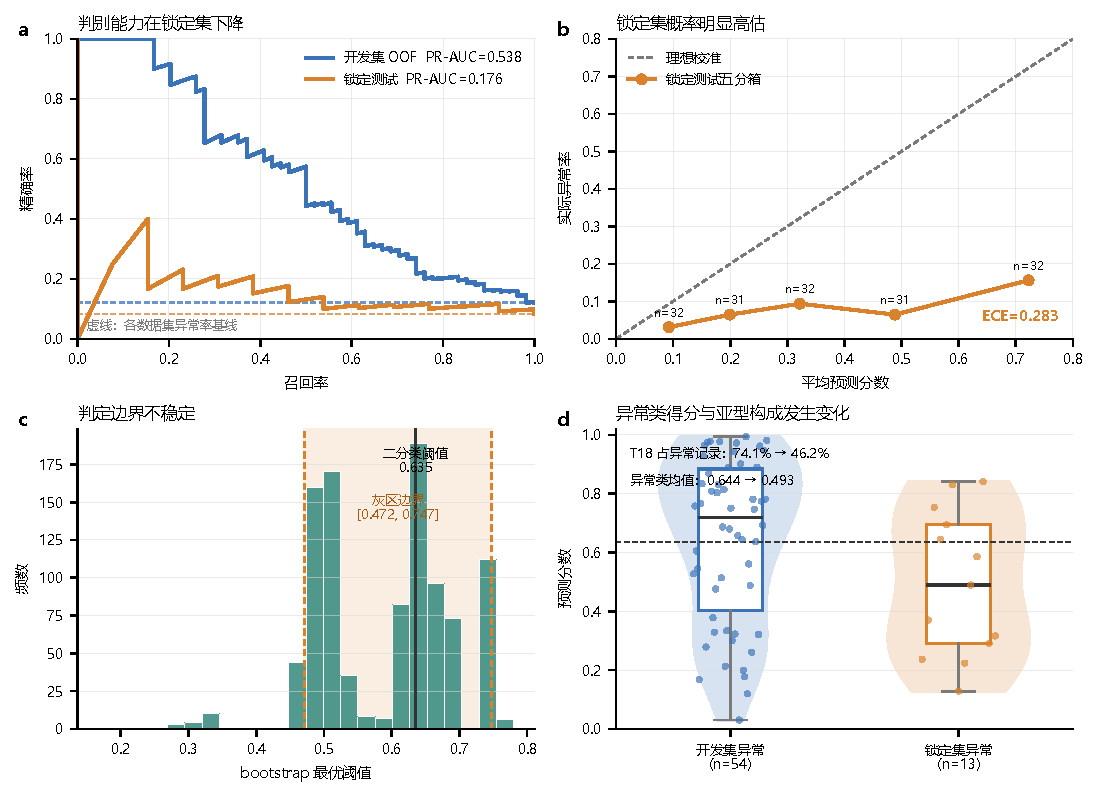
\includegraphics[width=\textwidth]{论文图表/q4_figure_1.pdf}
			\caption{问题四判别、校准、阈值不确定性与泛化误差诊断。a：开发集OOF与锁定测试PR曲线，虚线为各自异常率基线；b：锁定测试五分箱校准曲线；c：1000次孕妇级bootstrap阈值分布，橙色区域为$[0.471680,0.747108]$灰区边界；d：开发集与锁定集异常记录的得分分布，并标注T18构成变化。}
			\label{fig:q4_performance_diagnostics}
			\end{figure}

			\subsection{误差分析}
			\subsubsection{开发集与测试集结构问题}
			两组中“曾出现AB异常”的孕妇比例接近，开发集为0.3000，锁定集为0.2973，但记录级结构并未随之平衡。开发集异常记录率为0.1208，锁定集仅为0.0823；在曾异常孕妇内部，异常记录比例由0.4060降至0.2549。亚型构成也有变化：异常记录中的T18占比由0.7407降至0.4615，T21占比则由0.1667升至0.3077。现有外层分层保证了异常孕妇人数，却没有同时约束每名孕妇的记录负担和亚型比例，这与模型的记录级预测目标并不完全匹配。

			得分分布进一步说明差异集中在少数类。全部记录的平均预测分数在开发集和锁定集分别为0.3686和0.3652，正常记录也只从0.3308变为0.3537；异常记录的均值却从0.6437降至0.4927。故泛化下降不能简单归因于整体人群平移，主要变化发生在异常记录的条件分布中。

			\subsubsection{小规模验证与问题复现}
			为判断当前外层划分是否只源于程序错误，保持“按孕妇分组、按是否曾异常分层、37人进入锁定集”的规则不变，重新随机划分10000次。实际锁定集异常记录数不超过13条的频率为4.21\%，记录异常率差不小于当前值的频率为3.55\%，曾异常孕妇内部异常记录比例差不小于当前值的频率为1.59\%。记录率差与T18构成差同时达到当前程度的频率为0.27\%。这些数值是看到锁定结果后的描述性Monte Carlo尾频，用于复现结构问题，不能解释为预注册显著性检验的$p$值，也不能据此更换随机种子。

			异常率降低会机械压低PR-AUC。将开发集和锁定集的PR-AUC调整到相同异常率后，两者仍分别为0.472686和0.242117，相差约0.23，说明患病率差只能解释部分落差。保持正式划分不变的事后对照中，M0、M1和M2的锁定PR-AUC分别为0.083520、0.182914和0.175606；M1略高于M2，但这项比较发生在锁定结果揭示之后，只能说明GC增量没有稳定迁移，不能作为改选M1的依据。

			\subsubsection{误差结构分析与结论}
			条件分布检查发现，异常类$Z_{18}$的开发集--锁定集标准化均值差为$-0.823$，多个GC变量的单变量判别方向也发生翻转。开发集中$G_{13}$、$G_{18}$和$G_{21}$的两两相关系数绝对值为0.977至0.989，标准化设计矩阵条件数为19.25。M2在开发集识别出的GC增量因此容易受到亚型构成和小样本波动影响，这是锁定集上M1与M2接近的主要统计解释。

			标签本身也限制了模型上限。44名曾异常孕妇中有43名同时存在AB空白记录，32个同次复测组中有5组标签不一致，AB更像带测量波动的单次筛查结果。类别加权还使两组平均预测分数均约为0.37，明显高于实际异常率0.1208和0.0823，造成校准偏移。相比之下，年份、采血次数和孕周等整体协变量差异较小，目前没有证据把粗粒度时间漂移列为主因。

			综合这些检查，泛化误差由有限异常样本、记录负担与亚型构成变化、异常类条件特征漂移、GC共线性和代理标签噪声共同造成。正式模型和阈值保持不变，但其适用范围缩小为当前附件平台下的AB标签复现；若获得新的独立异常孕妇，应采用同时约束异常记录负担与T13/T18/T21构成的前瞻性分层，并在独立校准集上重新校准概率。
			
			\subsection{第四问结论}
			问题四可按以下步骤操作。对一条新的女胎检测记录，先按附件口径取得$Z_{13}$、$Z_{18}$、$Z_{21}$、$Z_X$、X染色体浓度以及总体和三条目标染色体的GC含量；若核心字段缺失或计量口径不同，则不直接套用模型。将这些变量代入式\eqref{eq:q4_final_score}和式\eqref{eq:q4_final_probability}得到异常分数$p$，再按式\eqref{eq:q4_three_way_rule}输出：$p<0.471680$判为正常倾向，$p>0.747108$判为异常倾向，中间区间标记为灰区并建议复核。若评价环节必须给出二分类结果，则以$p\ge0.635314$作为异常线，但该阈值不替代灰区规则。

			T13和T18可以在主判定之后给出条件式辅助提示，T21因样本不足只报告探索结果。对于极端测序质量记录，现有样本不能支持统一的自动拒判阈值，应保留质量标记并转人工复核。该方法在开发集内能够识别AB异常相关信号，但锁定测试PR-AUC为0.175606、召回率为0.384615，不能用于临床确诊，也不宜在新平台上直接外推。它回答了题目所需的可执行判定方法，同时把不确定记录和模型失效边界显式保留下来。

			\section{结论}
			%文章主结论，最后正面回应题目要求
			本文以孕妇级划分和锁定测试贯穿四问，得到的题目输出如下。
			\begin{enumerate}[label=\arabic*),leftmargin=2.2em,itemsep=4pt,topsep=3pt]
			\item \textbf{Y染色体浓度关系模型。}采用式\eqref{eq:q1_mundlak_model}的Mundlak组内--组间模型。同一孕妇内孕周每增加1周，Y浓度平均增加0.003203，95\%置信区间为$[0.002612,0.003794]$，Holm校正$p<0.001$；孕妇间平均BMI每增加$1\,\mathrm{kg/m^2}$，Y浓度平均降低0.001819，95\%置信区间为$[-0.003303,-0.000336]$，校正$p=0.049$。个体内BMI及孕周与BMI交互项不显著。锁定测试中核心方向保持一致，但$R^2$约为0.2，故模型回答相关特性和显著性，不用于预测个人精确浓度。
			\item \textbf{问题二的BMI分组与最佳时点。}BMI输出为$<30$、$[30,35)$和$\geq35$三个风险沟通层。四种数据分区、500次选择bootstrap和固定粗分层的one-SE比较均未支持组间系数，因此三组采用同一策略。基准情景下，三组均在10.5周首检，失败后于11.0周重检，累计可靠结果概率为0.9009，期望检测次数为1.1905。192个预设情景中136个可行，条件最优首检周为10--22.5周；只有56个情景达到稳定标准。检测误差和条件二次成功因子会改变可行性与推荐周数，但未产生稳定的BMI组间差异。
			\item \textbf{问题三的多因素分组与时点。}年龄、身高、体重、受孕方式和孕产史均已进入增量比较；检测前最佳候选的Brier分数改善2.06\%，未达到3\%保留线，条件重检模型虽平均改善17.08\%，最差折却恶化28.48\%。因此最终仍采用上述三个BMI层和式\eqref{eq:q3_final_probability}的共用概率曲线。基准情景输出仍为10.5周首检、11.0周重检，直接达标比例0.8343，累计可靠概率0.9009；其余情景给出10--22.5周的条件范围或报告不可行。该结果表示新增因素在本样本中不足以改变策略，不表示它们在其他人群中无效。
			\item \textbf{女胎异常判定方法。}将$Z_{13}$、$Z_{18}$、$Z_{21}$、$Z_X$、X染色体浓度及总体和三条目标染色体的GC含量代入式\eqref{eq:q4_final_score}，再由式\eqref{eq:q4_final_probability}得到异常分数$p$。若$p<0.471680$，输出正常倾向；若$p>0.747108$，输出异常倾向；中间区间标记为灰区并复核。必须二分类时采用$p\geq0.635314$作为异常线。锁定测试PR-AUC为0.175606、召回率为0.384615，故该方法只能作为当前附件平台的AB标签复现规则，不能替代临床诊断或直接迁移到新平台。
			\end{enumerate}
		
		%模型评价与推广	
			\section{模型推广与评价}
			\subsection{模型优点}
			%正确处理了什么问题，有什么创新行性
			本文在研究设计阶段纳入重复测量结构，并据此计算聚类稳健标准误。同一孕妇及技术复测组不跨训练、验证和测试集合，问题一分离组内与组间效应，问题二、三对删失达标信息和检测误差分别建模。这样处理避免了把记录数误当作独立样本量，也使每个输出都能对应到新孕妇的验证结果。

			时点模型将达标概率与决策风险分成两层。概率模型只负责估计附件可支持的规律，检测次数、累计可靠性、延迟和错误接受再进入有限网格优化。题目没有提供的临床损失和重检成功率不被固定为单一常数，而是通过192个预设情景和联合bootstrap报告条件解、范围或不可行。第三问在增量证据不足时保留冻结基线，没有为了形式上的“多因素”而增加不稳定变量。

			女胎模型也保留了失败边界。逐级特征块、重复分组验证和$L_2$惩罚限制了小样本下的自由度；阈值bootstrap将23.04\%的开发记录划入灰区。锁定测试性能下降后，模型和阈值没有按测试结果重新选择，而是如实缩小适用范围。
			\subsection{模型局限}
			%在什么地方上，由于什么原因，没有达到
			数据来自单一地区和单一附件平台，且样本以高BMI孕妇为主。BMI两端人数少，问题二、三很难识别细切点；问题四只有147名女胎孕妇，异常记录更少，AB标签还存在同次复测不一致。因此，当前分组和阈值不能视为跨地区、跨平台的临床标准。

			题目未提供完整的no-call字段、重抽结局、临床误判代价和独立确诊标签。文中的$a$、$b$和$\rho$是附件内部代理或情景参数，$J_g$也是无量纲决策损失。问题一的固定效应只能解释约两成记录级波动，问题四锁定测试的PR-AUC和召回率较低；这两部分分别限制了个体浓度预测和女胎异常筛查的强结论。

			锁定测试虽然以孕妇为单位分层，却没有同时约束异常记录负担及T13、T18、T21的亚型构成。问题四的异常类条件分布发生变化，加之GC变量高度共线，开发集中的增量未能稳定迁移。现有锁定集规模也不足以完成可靠的外部校准。
			\subsection{模型推广}
			%可以参考什么，哪些应该慎重，
			本文的“纵向关系估计--达标概率--条件决策”框架可以用于其他具有重复检测和阈值达标任务的生物标志物。推广时应重新定义可靠阈值、时间损失和重检路径，并在目标人群中重新估计概率曲线；原样移植本研究的10.5周时点没有统计依据。

			若获得更完整的随访数据，可用联合纵向--事件模型直接连接Y浓度轨迹与首次可靠结果，并以真实重抽结局估计条件二次成功率\citeup{11}。女胎异常判定则需要增加独立异常孕妇，按记录负担和非整倍体亚型前瞻性分层，在独立校准集上重新估计截距与阈值。达到外部验证标准之前，灰区记录和极端质量记录均应保留人工复核，不应自动给出临床诊断。
		}
	\end{spacing}
	
	\newpage
	
	%附录部分
	
	% 参考文献部分
	\section{参考文献}

	
	\begin{spacing}{1.25} % 1.25 倍行距
		\zihao{5}             % 五号字
	\sloppy
	\begin{enumerate}[label={[\arabic*]}, leftmargin=2em, labelwidth=1.5em, labelsep=0.5em, itemsep=0pt, parsep=0pt, partopsep=0pt, topsep=0pt]		
		\item ROLNIK D L, YONG Y, LEE T J, et al. Influence of Body Mass Index on Fetal Fraction Increase With Gestation and Cell-Free DNA Test Failure[J]. Obstetrics \& Gynecology, 2018, 132(2): 436--443. DOI:10.1097/AOG.0000000000002752.
		\item AMERICAN COLLEGE OF OBSTETRICIANS AND GYNECOLOGISTS, AMERICAN INSTITUTE OF ULTRASOUND IN MEDICINE, SOCIETY FOR MATERNAL-FETAL MEDICINE. Methods for Estimating the Due Date: Committee Opinion No. 700[EB/OL]. 2017, reaffirmed 2025[2026-08-15]. https://www.acog.org/clinical/clinical-guidance/committee-opinion/articles/2017/05/methods-for-estimating-the-due-date.
		\item TURNBULL B W. The empirical distribution function with arbitrarily grouped, censored and truncated data[J]. Journal of the Royal Statistical Society: Series B (Methodological), 1976, 38(3): 290--295. DOI:10.1111/j.2517-6161.1976.tb01597.x.
		\item RINK B D, DUGOFF L, KULLER J A, et al. Society for Maternal-Fetal Medicine Consult Series \#74: Cell-free DNA screening for aneuploidies: Updated guidance[J/OL]. Pregnancy, 2025, 1: e70139[2026-08-15]. DOI:10.1002/pmf2.70139.
		\item MUNDLAK Y. On the pooling of time series and cross section data[J]. Econometrica, 1978, 46(1): 69--85. DOI:10.2307/1913646.
		\item LIANG K Y, ZEGER S L. Longitudinal data analysis using generalized linear models[J]. Biometrika, 1986, 73(1): 13--22. DOI:10.1093/biomet/73.1.13.
		\item WANG E, BATEY A, STRUBLE C, et al. Gestational age and maternal weight effects on fetal cell-free DNA in maternal plasma[J]. Prenatal Diagnosis, 2013, 33(7): 662--666. DOI:10.1002/pd.4119.
		\item ALTMAN D G, ROYSTON P. The cost of dichotomising continuous variables[J]. BMJ, 2006, 332(7549): 1080. DOI:10.1136/bmj.332.7549.1080.
		\item BENNETTE C, VICKERS A. Against quantiles: categorization of continuous variables in epidemiologic research, and its discontents[J]. BMC Medical Research Methodology, 2012, 12: 21. DOI:10.1186/1471-2288-12-21.
		\item BENN P, VALENTI E, SHAH S, et al. Factors associated with informative redraw after an initial no result in noninvasive prenatal testing[J]. Obstetrics \& Gynecology, 2018, 132(2): 428--435. DOI:10.1097/AOG.0000000000002728.
		\item RIZOPOULOS D, TAYLOR J M G, VAN ROSMALEN J, et al. Personalized screening intervals for biomarkers using joint models for longitudinal and survival data[J]. Biostatistics, 2016, 17(1): 149--164. DOI:10.1093/biostatistics/kxv031.
		\item AMERICAN COLLEGE OF OBSTETRICIANS AND GYNECOLOGISTS. Screening for Fetal Chromosomal Abnormalities[EB/OL]. (2026-01)[2026-08-16]. https://www.acog.org/clinical/clinical-guidance/practice-advisory/articles/2026/01/screening-for-fetal-chromosomal-abnormalities.
		\item HOPKINS M K, KOELPER N, CALDWELL S, et al. Obesity and no call results: optimal timing of cell-free DNA testing and redraw[J]. American Journal of Obstetrics and Gynecology, 2021, 225(4): 417.e1--417.e10. DOI:10.1016/j.ajog.2021.04.212.
		\item CHEN E Z, CHIU R W K, SUN H, et al. Noninvasive prenatal diagnosis of fetal trisomy 18 and trisomy 13 by maternal plasma DNA sequencing[J]. PLoS ONE, 2011, 6(7): e21791. DOI:10.1371/journal.pone.0021791.
		\item BOSSUYT P M, REITSMA J B, BRUNS D E, et al. STARD 2015: an updated list of essential items for reporting diagnostic accuracy studies[J]. BMJ, 2015, 351: h5527. DOI:10.1136/bmj.h5527.
		\item COLLINS G S, REITSMA J B, ALTMAN D G, et al. Transparent reporting of a multivariable prediction model for individual prognosis or diagnosis (TRIPOD): the TRIPOD statement[J]. BMJ, 2015, 350: g7594. DOI:10.1136/bmj.g7594.
		\item FAN H C, BLUMENFELD Y J, CHITKARA U, et al. Noninvasive diagnosis of fetal aneuploidy by shotgun sequencing DNA from maternal blood[J]. Proceedings of the National Academy of Sciences of the United States of America, 2008, 105(42): 16266--16271. DOI:10.1073/pnas.0808319105.
		\item PALOMAKI G E, DECIU C, KLOZA E M, et al. DNA sequencing of maternal plasma reliably identifies trisomy 18 and trisomy 13 as well as Down syndrome: an international collaborative study[J]. Genetics in Medicine, 2012, 14(3): 296--305. DOI:10.1038/gim.2011.73.
		\item STRAVER R, SISTERMANS E A, HOLSTEGE H, et al. WISECONDOR: detection of fetal aberrations from shallow sequencing maternal plasma based on a within-sample comparison scheme[J]. Nucleic Acids Research, 2014, 42(5): e31. DOI:10.1093/nar/gkt992.
		\item KIM S K, HANNUM G, GEIS J, et al. Determination of fetal DNA fraction from the plasma of pregnant women using sequence read counts[J]. Prenatal Diagnosis, 2015, 35(8): 810--815. DOI:10.1002/pd.4615.
	\end{enumerate}
	\end{spacing}
	
	%附录部分
	%创建appendix文档 
	
	%附录A AI使用声明 
	%appendix_AI_declaration AI使用声明
	
	%附录B 重要数据集
	%appendix_data    重要的长表数据，还有正文没有直接出现的重要数据，注意给出使用的地方
	
	%附录C 代码文件
	%appendix_contents 支撑文件目录，给出文件名和用途
	%appendix_code     代码文件
\end{document}

